\mathversion{sans}

\begin{quote}
\textit{Beware of bugs in the above code; I have only proved it correct, not tried it.}

\hfill Donald Knuth
\end{quote}

The correctness proofs in Chapters~\ref{ch:preimage1} and~\ref{ch:preimage2} assume an idealized model of the host language.
While Dr. Bayes's core is nearly a transliteration of the \lzfclang terms that define the approximating semantics, we cannot know how well the theorems apply to Dr. Bayes without testing it.

Besides, we must still demonstrate that it is useful.

\section{Guaranteed Termination}

The theorems in Chapter~\ref{ch:preimage1} require a program or expression $\mathit{e}$ to be well-defined (Definition~\ref{def:well-defined-expression}); in particular, any interpretation $\meaningofconv{\mathit{e}}\genc$ must terminate.
The syntax transformers that implement $\meaningofconv{\cdot}\genc$ and Racket's rules for module-level definitions enforce this.
For example, the following program is not well-defined according to the semantics:
\begin{center}\singlespacing
\begin{schemedisplay}
(define/drbayes (loop) (loop))
\end{schemedisplay}
\end{center}
Further, Racket raises a compile-time error, or more precisely, an expansion-time error.
Its interpretation as a bottom* arrow computation is
\begin{center}\singlespacing
\begin{schemedisplay}
(define loop/bot* (apply/bot* loop/bot* (list)))
\end{schemedisplay}
\end{center}
where \scheme{apply/bot*} composes a first-order function's interpretation with a list of argument interpretations.
(Here, the list is empty because there are no arguments.)
Racket's expander does not allow module-level bindings such as \scheme{loop/bot*} to be referenced except by subsequent module-level expressions and expressions in the bodies of lambdas.

On the other hand, this program is well-defined according to the semantics because its recurrences are guarded by $if$:
\begin{center}\singlespacing
\begin{schemedisplay}
(define/drbayes (loop) (if #t (loop) (loop)))
\end{schemedisplay}
\end{center}
Further, Racket raises no errors.
As a bottom* arrow computation, it is
\begin{center}\singlespacing
\begin{schemedisplay}
(define loop/bot*
  (ifte*/bot* (const/bot* #t)
              (lazy/bot* (delay (apply/bot* loop/bot* (list))))
              (lazy/bot* (delay (apply/bot* loop/bot* (list))))))
\end{schemedisplay}
\end{center}
Racket allows this definition of \scheme{loop/bot*} because the inner reference to \scheme{loop/bot*} is within a \scheme{delay} form, which expands to a lambda.
(A \scheme{(delay e)} in Racket is similar to $\fun{0} \mathit{e}$ in \lzfclang, but it caches the value of \scheme{e} when it is first computed, and is applied using \scheme{force}.)

To test termination guarantees, we exhibit a few programs with different termination conditions.
The first program never terminates:
\begin{center}\singlespacing
\begin{schemedisplay}
(define/drbayes never-terminate (loop))
\end{schemedisplay}
\end{center}
When asked for any number of samples in the preimage of any nonempty set, Dr. Bayes simply returns no samples:
\begin{center}\singlespacing
\begin{schemedisplay}
> (drbayes-sample never-terminate 100 univ-set)
'()
\end{schemedisplay}
\end{center}
How long sampling takes depends on the probability with which $\bot$ is chosen for branches: a lower probability of $\bot$ increases the average number of loops before $\bot$ is chosen, resulting in longer wait times.
Any probability of $\bot$ below $\frac{1}{3}$ seems reasonable, and we generally use $\frac{1}{5}$.

The following program returns \scheme{0} with probability $\frac{1}{2}$, and otherwise loops forever:
\begin{center}\singlespacing
\begin{schemedisplay}
(define/drbayes half-terminate
  (if (< (random) 1/2) 0 (loop)))
\end{schemedisplay}
\end{center}
With the probability of $\bot$ branches at $\frac{1}{5}$ and the probabilities of $true$ and $false$ at $\frac{2}{5}$, we should expect perhaps $\frac{2}{5}$ of the samples we ask for.
However, we get almost all of them:
\begin{center}\singlespacing
\begin{schemedisplay}
> (length (drbayes-sample half-terminate 500 univ-set))
486
\end{schemedisplay}
\end{center}
This is due to the self-adjusting tree search.
Each $\bot$ branch choice in the fully inlined \scheme{(loop)} results in an empty preimage, so its corresponding leaf in the search tree is removed.
The required adjustments reduce the probability the sampler chooses $false$ for \scheme{(< (random) 1/2)} in subsequent samples.

Roughly, the self-adjusting search ``learns'' that \scheme{(loop)} terminates with low probability and usually avoids it.
The more samples are taken, the lower its probability estimate, though it never reaches zero.

With probability $1$, the following program returns a geometrically distributed value.
\begin{center}\singlespacing
\begin{schemedisplay}
(define/drbayes (geometric p)
  (if (< (random) p) 0 (+ 1 (geometric p))))
<blank-line>
(define/drbayes almost-surely-terminate
  (geometric 1/2))
\end{schemedisplay}
\end{center}
Dr. Bayes rejects some samples:
\begin{center}\singlespacing
\begin{schemedisplay}
> (length (drbayes-sample almost-surely-terminate 500 univ-set))
493
\end{schemedisplay}
\end{center}
The rejected samples are from $\bot$ branch choices.
As with \scheme{half-terminate}, the self-adjusting search keeps the number of $\bot$ choices small.

This program always terminates, but abstractly does not seem to:
\begin{center}\singlespacing
\begin{schemedisplay}
(define/drbayes abstractly-loop
  (let ([x (random)]
        [y (random)])
    (if (< x y)
        (if (>= x y) (loop) 0)
        (if (< x y) (loop) 1))))
\end{schemedisplay}
\end{center}
When \scheme{(< x y)}, \scheme{(>= x y)} is impossible, so the program returns \scheme{0}.
Otherwise, \scheme{(< x y)} is impossible, so the program returns \scheme{1}.
Because \scheme{loop} is never applied, the program terminates.

However, the exact preimage of \scheme{true-set} under the interpretation of \scheme{(< x y)} cannot be represented directly; its rectangular cover is \scheme{univ-omega-set}.
The same is true for the exact preimage of \scheme{true-set} under \scheme{(>= x y)}.
In general, Dr. Bayes's implementation of $sample!part$ can never rule out all branch choices that lead to \scheme{(loop)}.

Because $sample!part$ may choose $\bot$ for a branch choice, sampling terminates anyway, though for sequences of choices that contain $\bot$ it rejects the sample.
The proportion of samples accepted depends on how finely the program domain is partitioned.
Dr. Bayes has a parameter \scheme{drbayes-max-splits} that determines how many times each projection is split in half: if set to $n$, the size of each projection's partition is $2^n$.
When set to \scheme{0}, the partition whose cover is sampled from is that induced by the program's minimal branch traces $T_*$.
With no splits, Dr. Bayes accepts about half the samples:
\begin{center}\singlespacing
\begin{schemedisplay}
> (drbayes-max-splits 0)
> (length (drbayes-sample abstractly-loop 500 univ-set))
235
\end{schemedisplay}
\end{center}
When set to a larger number, however, splitting the program domain allows preimage refinement to often determine that \scheme{(< x y)} implies not \scheme{(>= x y)}:
\begin{center}\singlespacing
\begin{schemedisplay}
> (drbayes-max-splits 5)
> (length (drbayes-sample abstractly-loop 500 univ-set))
480
\end{schemedisplay}
\end{center}
The only rectangular part covers that allow a later $\bot$ branch choice are those that contain $\omega$ for which \scheme{(< x y)} is true and others for which it is false; i.e. they straddle the line $\omega~j_x = \omega~j_y$ where $j_x$ and $j_y$ are the subcomputation indexes of the interpretations of each \scheme{(random)}.

Most of the examples so far require the possibility of $\bot$ branch choices to terminate.
However, most programs, like \scheme{almost-surely-terminate}, abstractly terminate with probability $1$, and thus do not require it.
Therefore, we define a parameter \scheme{drbayes-always-terminate?} and implement $sample!part$ so that it chooses $\bot$ only when \scheme{drbayes-always-terminate?} is set to \scheme{#t}.
For example,
\begin{center}\singlespacing
\begin{schemedisplay}
> (drbayes-always-terminate? #f)
> (length (drbayes-sample almost-surely-terminate 500 univ-set))
500
\end{schemedisplay}
\end{center}
The default value is \scheme{#f}.

\section{Primitives}

The last chapter demonstrates sampling in a preimage under subtraction (Figure~\ref{fig:sample-source}).
Addition is no more difficult.
In fact, by Theorem~\ref{thm:axial-inverse-cyclic-group}, once we have addition or subtraction it is easy to define the other so that it is just as efficient, because each is an axial inverse of the other.
Alternatively, we could define one from the other using an additional negation primitive and $a - b = a + (-b)$ or $a + b = a - (-b)$.

To help ensure Dr. Bayes is useful, it additionally has comparison primitives, multiplication and division primitives (for which one is easily defined in terms of the other), and various $\Re \pto \Re$ function primitives such as inverse cumulative distribution functions (CDFs) for a few common distributions.

When subtraction and predicates are defined, comparing real numbers is easy.
For example, if \scheme{negative?} is defined as in~\eqref{eqn:negative-pre}, then because $a < b$ if and only if $a - b < 0$,
\begin{center}\singlespacing
\begin{schemedisplay}
(define/drbayes (< a b)
  (negative? (- a b)))
\end{schemedisplay}
\end{center}
The other comparison operators are defined similarly.
We could define real equality by
\begin{center}\singlespacing
\begin{schemedisplay}
(define/drbayes (= a b)
  (and (<= a b) (<= b a)))
\end{schemedisplay}
\end{center}
However, real equality is rarely useful because \scheme{(= a b)} is usually a zero-probability event; i.e. the preimage of $\set{true}$ under the interpretation of \scheme{(= a b)} usually has zero measure.

\renewcommand{\subfigurewidth}{2.15in}
\begin{figure*}[tb!]\centering%
\subfloat[Preimage of {$[-0.1,0.2]$} under the interpretation of $(uniform~{-1}~1) \cdot (uniform~{-1}~1)$]{%
\label{fig:arithmetic-preimages:mul}%
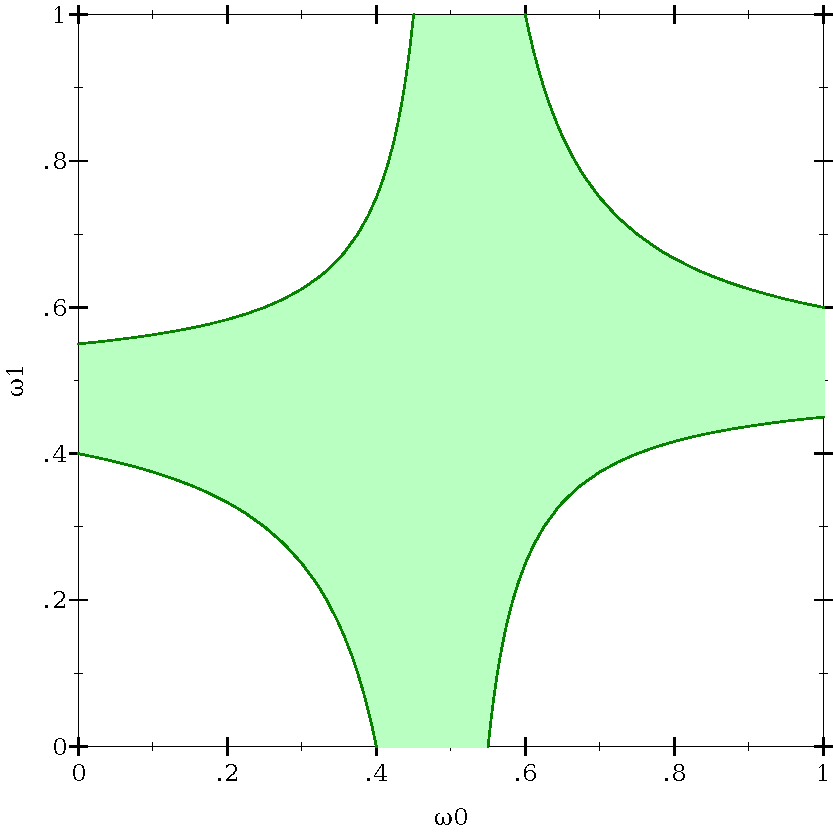
\includegraphics[width=\subfigurewidth]{figures/mul-preimage}%
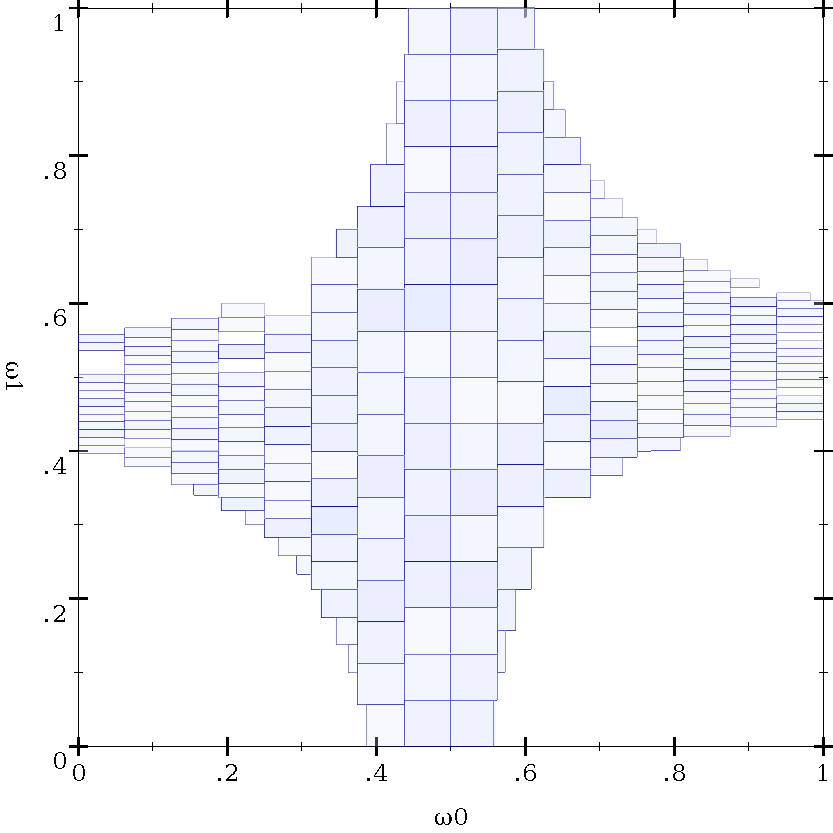
\includegraphics[width=\subfigurewidth]{results/mul-preimage-rects}%
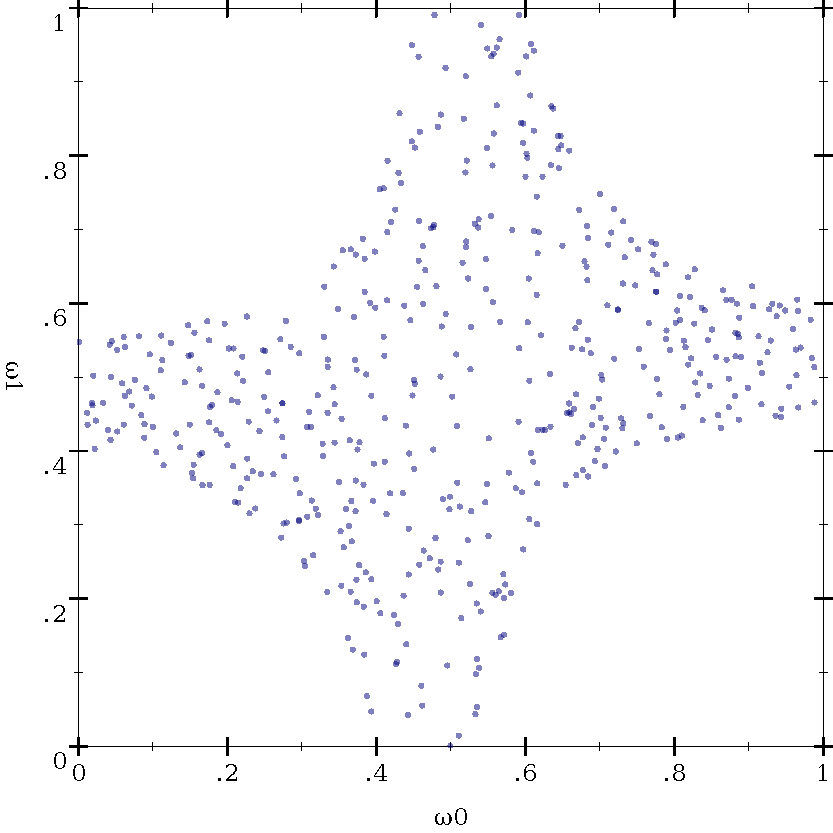
\includegraphics[width=\subfigurewidth]{results/mul-preimage-points}%
}

\subfloat[Preimage of {$[-0.5,1]$} under the interpretation of $(uniform~{-1}~1)~{/}~(uniform~{-1}~1)$]{%
\label{fig:arithmetic-preimages:div}%
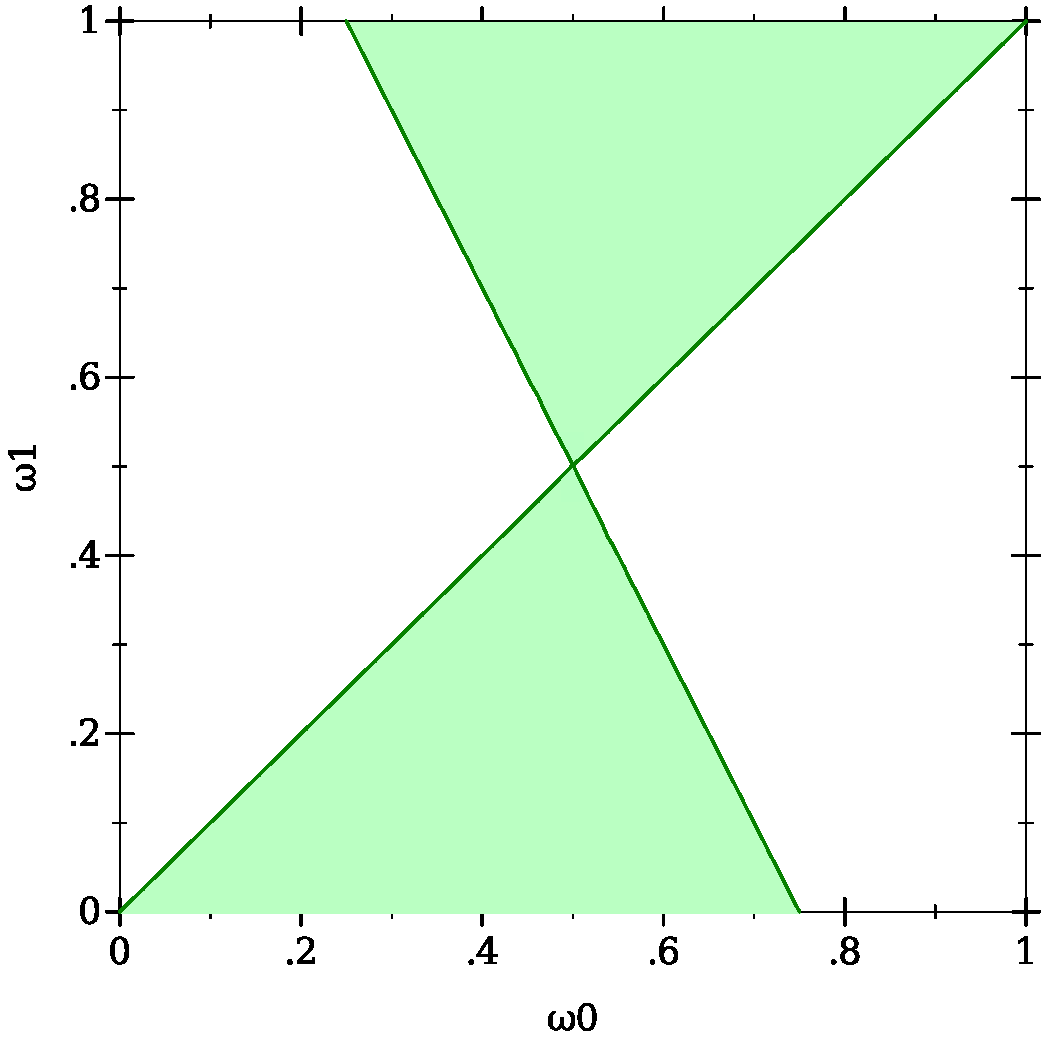
\includegraphics[width=\subfigurewidth]{figures/div-preimage}%
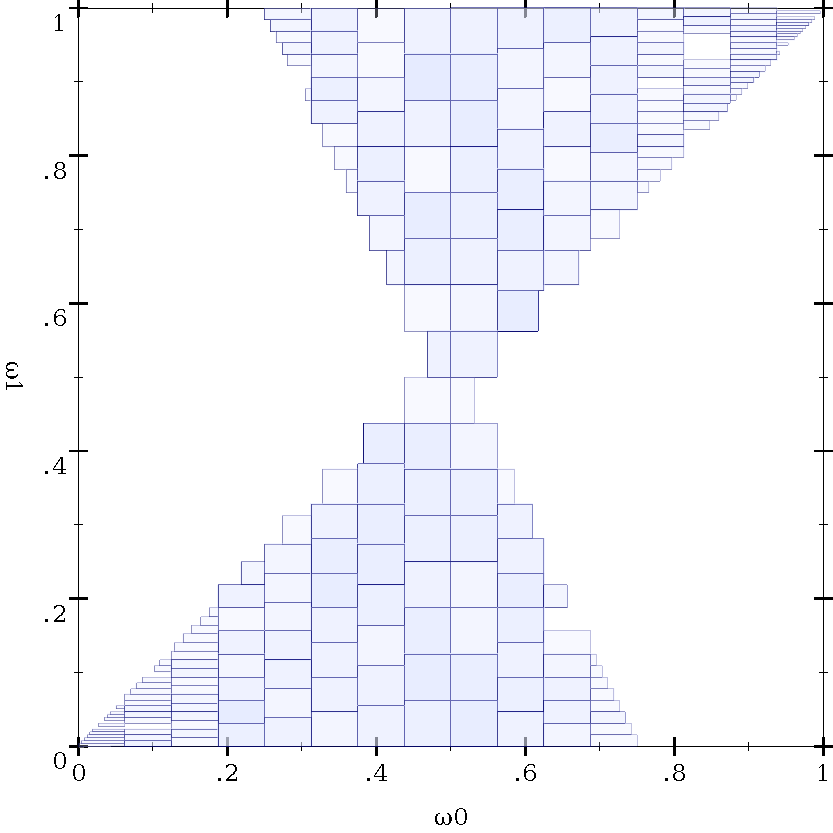
\includegraphics[width=\subfigurewidth]{results/div-preimage-rects}%
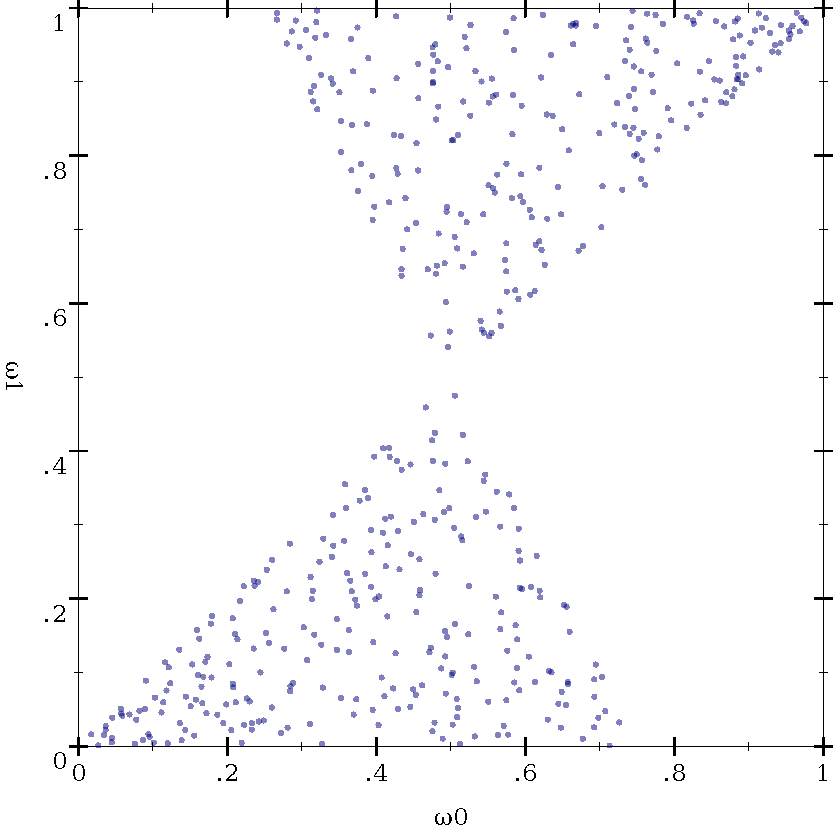
\includegraphics[width=\subfigurewidth]{results/div-preimage-points}%
}
\caption[Sampling from preimages under multiplication and division]{Exact preimages under multiplication and division, sampled part covers, and sampled points.}%
\label{fig:arithmetic-preimages}
\end{figure*}

Figure~\ref{fig:arithmetic-preimages:mul} shows the result of sampling in the preimage of $[-0.1,0.2]$ under the interpretation of either of the following equivalent programs:
\begin{center}\singlespacing
\begin{minipage}{2.2in}
\begin{schemedisplay}
(define/drbayes uniform-mul
  (* (uniform -1 1)
     (uniform -1 1)))
\end{schemedisplay}
\end{minipage}
\hspace{0.5in}
\begin{minipage}{2.3in}
\begin{schemedisplay}
(define/drbayes uniform-mul
  (* (+ -1 (* 2 (random)))
     (+ -1 (* 2 (random)))))
\end{schemedisplay}
\end{minipage}
\vspace{\baselineskip}
\end{center}
Similarly, Figure~\ref{fig:arithmetic-preimages:div} shows the result of sampling in the preimage of $[-0.5,1]$ under the interpretation of \scheme{(/ (uniform -1 1) (uniform -1 1))}.

There are two points of interest here.
The first is that the point samples in Figure~\ref{fig:arithmetic-preimages} exhibit nonuniformity.
(It is in the horizontal arms in the multiplication preimage, and in the corners in the division preimage.)
Nonuniformity arises from the fact that the probabilities with which part covers are chosen can only approximate the covered parts' true measures (Figure~\ref{fig:preimage-refinement-sampling}), and from sampling dependent uniform random variables in $sample!source^*$~\eqref{eqn:sample-source*}.
It is adjusted for by weighting the samples, and is further mitigated by the extension to the self-adjusting search that causes the search tree to converge to a tree with stated leaf probabilities (Section~\ref{sec:self-adjusting}).
But nonuniformity can lower the samples' information content in a query-dependent way.
We quantify it further on.

The second point of interest is that \scheme{(uniform -1 1)} is defined by a function that encodes the \keyword{uniform distribution family}:
\begin{center}\singlespacing
\begin{schemedisplay}
(define/drbayes (uniform a b)
  (+ a (* (- b a) (random))))
\end{schemedisplay}
\end{center}
This function transforms uniform random variables on the unit interval into uniform random variables between \scheme{a} and \scheme{b}.
The uniform distribution family is one of the simplest common examples of a \keyword{location-scale family}, which can always be encoded in Dr. Bayes as
\begin{center}\singlespacing
\begin{schemedisplay}
(define/drbayes (family-name loc scale)
  (+ loc (* scale (standard-inv-cdf (random)))))
\end{schemedisplay}
\end{center}
For the uniform distribution family, \scheme{standard-inv-cdf} is the identity function.

Another location-scale family, the normal distribution family, is encoded in Dr. Bayes using the implementation of $normal!inv!cdf\pre$~\eqref{eqn:normal-inv-cdf-pre}:
\begin{center}\singlespacing
\begin{schemedisplay}
(define/drbayes (normal $\va{\mu}$ $\va{\sigma}$)
  (+ $\va{\mu}$ (* $\va{\sigma}$ (normal-inv-cdf (random)))))
\end{schemedisplay}
\end{center}
Other implemented families include the exponential, Cauchy, and logistic distribution families.

Some distribution families are significantly more difficult to encode.
For example, gamma distributions are parameterized on a \emph{shape} and a scale.
Because one parameter is a scale, we can reduce the work to implementing a two-argument primitive \scheme{gamma-inv-cdf}:
\begin{center}\singlespacing
\begin{schemedisplay}
(define/drbayes (gamma k $\va{\theta}$)
  (* $\va{\theta}$ (gamma-inv-cdf k (random))))
\end{schemedisplay}
\end{center}
Implementing \scheme{gamma-inv-cdf} requires implementing the following trijection, extended to a compact superdomain.
\begin{equation}
\begin{aligned}
	F_p &: (0,{+\infty}) \times (0,{+\infty}) \to (0,1) \hspace{0.5in}&& \text{Gamma CDF} \\
	F_x &: (0,{+\infty}) \times (0,1) \to (0,{+\infty}) && \text{Gamma inverse CDF} \\
	F_k &: (0,1) \times (0,+\infty) \to (0,{+\infty}) && \text{???}
\end{aligned}
\end{equation}
$F_p$ and $F_x$ are well-known, and Racket's \scheme{math/distributions} library exports quite accurate implementations of them.
Unfortunately, as far as we can tell, no one else has ever needed an implementation of $F_k$.
While the numerical analysis required to implement it accurately on its entire domain is beyond the scope of this work, we plan to do it in the future.

As soon as we have \scheme{gamma}, we can encode other distributions important in Bayesian modeling by encoding sampling algorithms for them that are defined in terms of gamma distributions.
For example, the inverse gamma and beta families can be encoded by
\begin{center}\singlespacing
\begin{schemedisplay}
(define/drbayes (inv-gamma k $\va{\theta}$)
  (/ 1 (gamma k $\va{\theta}$)))
<blank-line>
(define/drbayes (beta $\va{\alpha}$ $\va{\beta}$)
  (let ([x  (gamma $\va{\alpha}$ 1)]
        [y  (gamma $\va{\beta}$ 1)])
    (/ x (+ x y))))
\end{schemedisplay}
\end{center}
The Dirichlet distribution family encoding would be similar to \scheme{beta}, but would use structural recursion  over a list of parameters to get and normalize an unbounded number of gamma-distributed random variables.

In general, as with \scheme{beta}, the encoding of any sampling algorithm is also an encoding of the distribution or distribution family it samples from.
For example, this encoding of the Box-Muller algorithm~\cite{cit:box-1958-normal} also encodes the standard normal distribution:
\begin{center}\singlespacing
\begin{schemedisplay}
(define/drbayes (normal/box-muller)
  (* (sqrt (* -2 (log (random))))
     (partial-cos (* pi (uniform -1 1)))))
\end{schemedisplay}
\end{center}
Here, \scheme{partial-cos} is the cosine function defined on $[-\pi,\pi]$, which is implemented by pasting together two symmetric, monotone pieces defined on $[-\pi,0]$ and $[0,\pi]$.

Using \scheme{(normal-inv-cdf (random))} instead of \scheme{(normal/box-muller)} is much faster, consisting of one $\Omega$ projection and one primitive operation instead of two $\Omega$ projections and nine primitive operations.
However, the point of defining \scheme{(normal/box-muller)} is to demonstrate the expressive power of a probabilistic language defined measure-theoretically.

A language based on probability density functions necessarily distinguishes between primitive and derived random variables.
The former are simply projections, and conditions are restricted to be primitive random variable equalities so that conditional densities always exist.
Conditions referring to a derived random variable such as \scheme{(normal/box-muller)}, or even \scheme{(normal mu sigma)} using the present definition of \scheme{normal}, are close to unthinkable.

We will explore how to leverage this new expressiveness after showing how Bayesian theories with density models are encoded in Dr. Bayes, and showing how to use its sampling algorithm to answer conditional queries about them.

\section{Theories With Density Models}

\subsection{Normal-Normal}

We start with one of the simplest Bayesian theories, the normal-normal, introduced in Chapter~\ref{ch:background}.
Specified constructively, it is
\mathversion{normal}
\begin{equation}
\begin{aligned}
	X &\sim \mathrm{Normal}(0,1) \\
	Y &\sim \mathrm{Normal}(X,1)
\end{aligned}
\end{equation}
\mathversion{sans}
There are many possible encodings in Dr. Bayes whose interpretations are a model of this theory.
One of the most straightforward is
\begin{center}\singlespacing
\begin{schemedisplay}
(define/drbayes normal-normal
  (let* ([x  (normal 0 1)]
         [y  (normal x 1)])
    (cons x y)))
\end{schemedisplay}
\end{center}
where \scheme{let*} makes \scheme{x} visible in the definition of \scheme{y} by expanding to nested \scheme{let} expressions, and \scheme{cons} constructs pairs.

In Chapter~\ref{ch:background}, we used Bayes' law for densities to find the distribution of $\mathit{X}$ given $\mathit{Y} = 2$.
By not defining the language in terms of densities, we have given up the ability to handle such zero-probability conditions except as limits, and we cannot wait for limits to complete.
We will show that not having zero-probability conditions matters little.

But first, from a philosophical standpoint, the condition $\mathit{Y} = 2$ is hard to support: it is an assertion about \emph{all of the countably many digits} of $\mathit{Y}$.
If finding the distribution of $\mathit{X} \given \mathit{Y} = 2$ is a typical inference task, this amounts to having infinite knowledge about a real-world observation.
Still, zero-probability conditions are often convenient, so we intend to investigate supporting them in future work.

To sample within a positive-probability preimage, the condition needs to be wider; e.g. $\mathit{Y} \in [2-\varepsilon,2+\varepsilon]$ where $\varepsilon > 0$ is small.
For \scheme{normal-normal}, we must sample within the preimage of $\Re \times [2-\varepsilon,2+\varepsilon]$.
Equivalently, we could encode the condition in the program as a proposition about \scheme{y}:
\begin{center}\singlespacing
\begin{schemedisplay}
(define/drbayes normal-normal/cond
  (let* ([x  (normal 0 1)]
         [y  (normal x 1)])
    (cons x (<= (- 2 $\va{\varepsilon}$) y (+ 2 $\va{\varepsilon}$)))))
\end{schemedisplay}
\end{center}
and sample within the preimage of $\Re \times \set{true}$.

\renewcommand{\subfigurewidth}{2.15in}
\begin{figure*}[tb!]\centering%
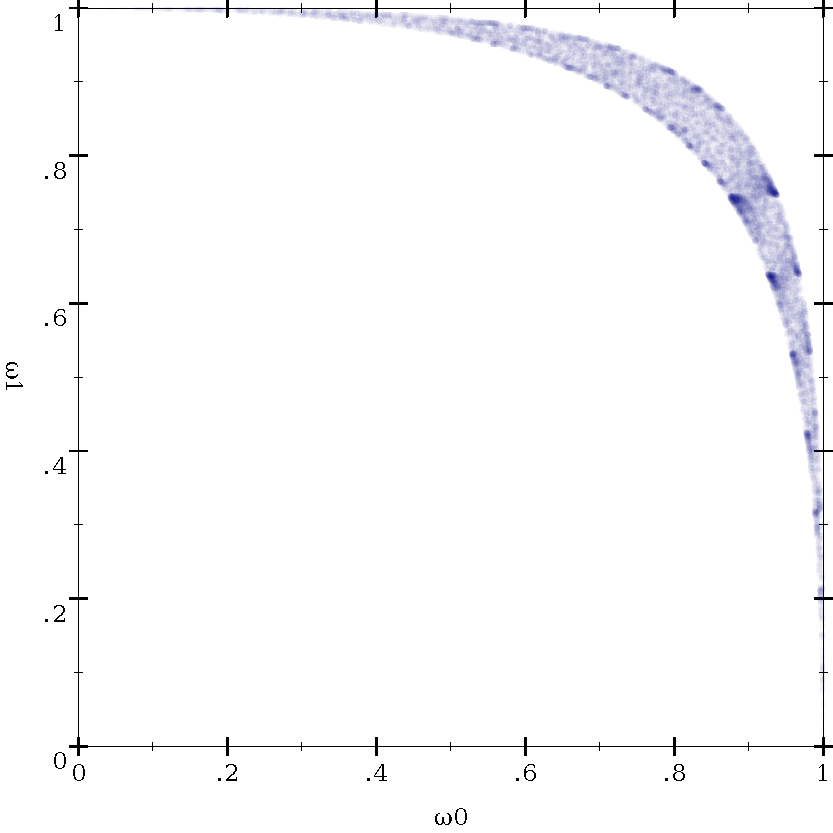
\includegraphics[width=\subfigurewidth]{results/normal-normal-2-points}%
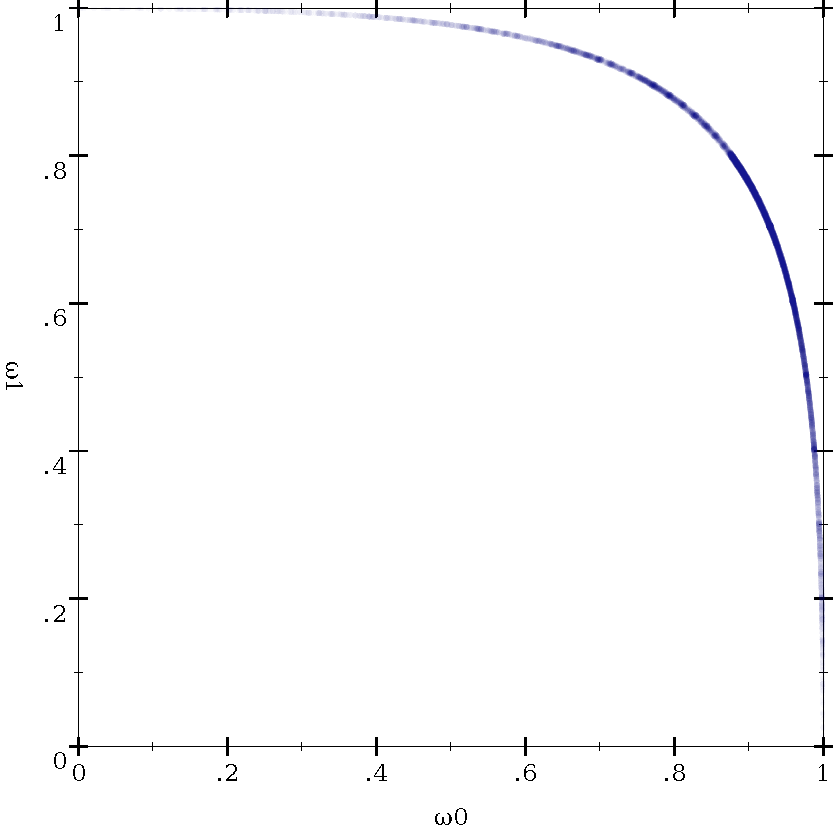
\includegraphics[width=\subfigurewidth]{results/normal-normal-01-points}%
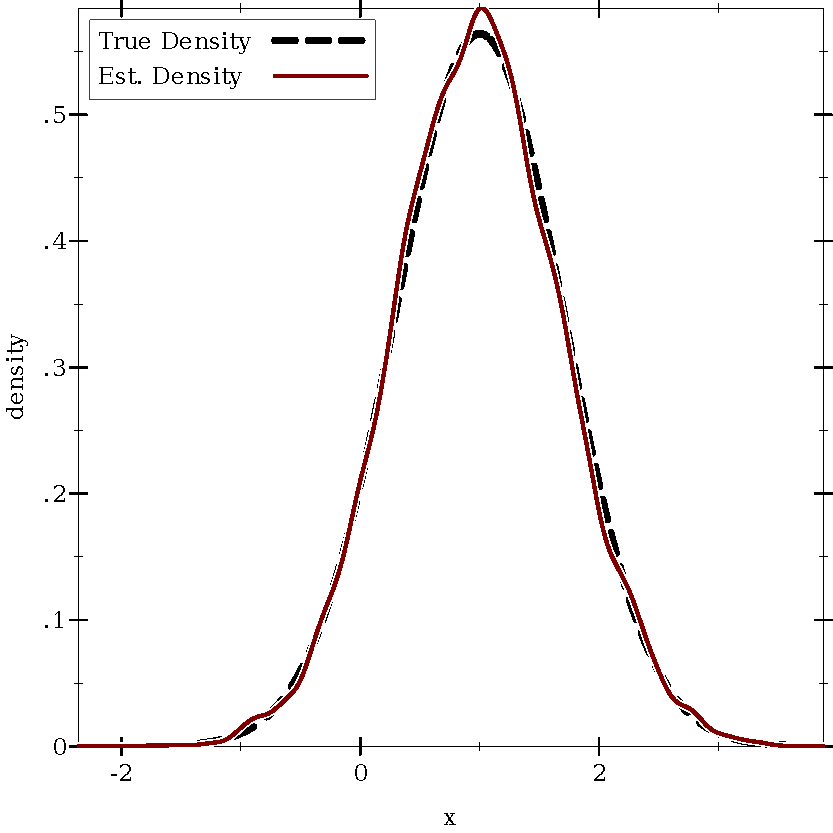
\includegraphics[width=\subfigurewidth]{results/normal-normal-density}%
\caption[Samples from Dr. Bayes and a density estimate]{From left to right, samples from the preimage of {$[1.8,2.2]$}, samples from the preimage of {$[1.99,2.01]$}, and a density estimate computed from the image of the first set of samples.}%
\label{fig:normal-normal}
\end{figure*}

Figure~\ref{fig:normal-normal} shows the results of sampling 10000 times within the preimage for $\varepsilon = 0.2$ and $\varepsilon = 0.01$, each of which takes about 3 seconds on current hardware.
The last plot is a density estimate of the distribution of $\mathit{X} \given \mathit{Y} \in [1.8,2.2]$, wherein $\varepsilon = 0.2$, not $0.01$.
Even so, the density estimate is very good (and is consistently so in multiple tests), suggesting that we do not need anything close to a zero-probability condition.
A fairly wide interval centered on $2$ is enough.

For $\varepsilon = 0.2$, sufficient statistics for the computed distribution are
\begin{center}\singlespacing
\begin{schemedisplay}
> (mean xs ws)
0.9883685519606158
<blank-line>
> (stddev xs ws)
0.7033198741144521
\end{schemedisplay}
\end{center}
where \scheme{xs} are the first of every sampled \scheme{(cons x y)}, and \scheme{ws} are the sample weights.
The exact values of these statistics for $\mathit{X} \given \mathit{Y} = 2$ are $1$ and $\sqrt{\frac{1}{2}} \approx 0.707107$.

Every value we estimate from samples, such as \scheme{(mean xs ws)} and \scheme{(stddev xs ws)}, is actually a random variable.
The standard way to quantify their uncertainty or information content is by estimating their variance, which is called \keyword{Monte Carlo variance}~\cite[Chapter~12]{cit:degroot-2012book-probability}.
To get Monte Carlo variance of the estimated mean \scheme{(mean xs ws)} in the same units as the mean, we use \scheme{mc-stddev} from Racket's \scheme{math/statistics} library, which returns the square root of an estimate of Monte Carlo variance, computed from the samples:
\begin{center}\singlespacing
\begin{schemedisplay}
> (mc-stddev xs ws)
0.007754889592107897
\end{schemedisplay}
\end{center}
We continue to follow DeGroot~\cite{cit:degroot-2012book-probability}.
By the Central Limit theorem, the distribution of \scheme{(mean xs ws)} should be approximately normal, and we have so many samples that we may simply fit a normal distribution to it to obtain a confidence interval:
\begin{center}\singlespacing
\begin{schemedisplay}
> (real-dist-hpd-interval
   (normal-dist (mean xs ws) (mc-stddev xs ws))
   0.95)
0.9731692476559998
1.0035678562652317
\end{schemedisplay}
\end{center}
Here, \scheme{real-dist-hpd-interval} finds the High Probability Density (HPD) interval: the narrowest interval containing $95\%$ of the area under the density of the distribution object returned by \scheme{normal-dist}.
Thus, we are $95\%$ confident that the mean of $\mathit{X} \given \mathit{Y} = 2$ is between $0.973$ and $1.004$.

In this example, weighted samples carry almost as much information as unweighted.
For comparison, here are the same results computed from 10000 unweighted samples chosen according to the exact distribution of $\mathit{X} \given \mathit{Y} = 2$:
\begin{center}\singlespacing
\begin{schemedisplay}
> (define zs (sample (normal-dist 1 (sqrt 1/2)) 10000))
<blank-line>
> (mean zs)
0.9969732989599994
<blank-line>
> (stddev zs)
0.7035825345789904
<blank-line>
> (mc-stddev zs)
0.0070358253457899035
<blank-line>
> (real-dist-hpd-interval
   (normal-dist (mean zs) (mc-stddev zs))
   0.95)
0.9831833346807372
1.0107632632392618
\end{schemedisplay}
\end{center}
Monte Carlo variance is a little lower, so the resulting confidence interval is a little tighter.

We can also compute probabilities as expected values, as discussed in Chapter~\ref{ch:countable-models}.
For example, $\Pspec{\mathit{X} \in (0,1) \given \mathit{Y} = 2}$ is approximately
\begin{center}\singlespacing
\begin{schemedisplay}
> (mean (map (indicator (λ (x) (< 0 x 1))) xs) ws)
0.42033680800148004
\end{schemedisplay}
\end{center}
where \scheme{indicator} converts $X \tto Bool$ functions into $X \tto \set{0,1}$ functions.
As with the mean, this computed probability is also a random variable, but fitting a normal distribution using Monte Carlo variance may be a bad idea: the fitted distribution would give positive probability to sets containing negative ``probabilities.''
It is better to fit a beta distribution, which has support only in $[0,1]$, and is well-suited for characterizing distributions over probabilities.
The \scheme{math/statistics} export \scheme{mc-prob-dist} does this for us:
\begin{center}\singlespacing
\begin{schemedisplay}
> (real-dist-hpd-interval
   (mc-prob-dist (λ (x) (< 0 x 1)) xs ws)
   0.95)
0.41066735830660506
0.4300151946469193
\end{schemedisplay}
\end{center}
Thus, we are $95\%$ confident that $\Pspec{\mathit{X} \in (0,1) \given \mathit{Y} = 2}$ is between about $0.41$ and $0.43$.

The following encoding of the same normal-normal theory uses the standard normal distribution as defined using the Box-Muller algorithm.
\begin{center}\singlespacing
\begin{schemedisplay}
(define/drbayes normal-normal/box-muller
  (let* ([x  (normal/box-muller)]
         [y  (+ x (normal/box-muller))])
    (cons x y)))
\end{schemedisplay}
\end{center}
The results (elided) from taking 10000 samples in the preimage of $[1.8,2.2]$ are nearly identical, except the Monte Carlo standard deviation is higher, at approximately $0.0115$ instead of $0.00775$, and collecting the samples takes about 22 seconds instead of 3.

\subsection{Normal-Normals}

Extending the normal-normal theory with more observations requires adding more random variables that depend on $\mathit{X}$.
A template for encoding them is
\begin{center}\singlespacing
\begin{schemedisplay}
(define/drbayes normal-normals
  (let ([x  (normal $\va{\mu}$ $\va{\sigma}$)])
    (list x (normal x $\va{\sigma_1}$) ... (normal x $\va{\sigma_n}$))))
\end{schemedisplay}
\end{center}
We sample within preimages of $\Re \times [y_1-\varepsilon_1,y_1+\varepsilon_1] \times ... \times [y_n-\varepsilon_n,y_n+\varepsilon_n] \times \set{\pair{}}$, where $y_1,...,y_n$ are the observed data.
(In functional languages, a finite list consists of nested pairs terminated by $\pair{}$.)
Each observation $y_i$ has its own interval width $\varepsilon_i$.

\begin{figure*}[tb!]\centering
\includegraphics[width=3in]{figures/nested-rectangles}
\caption[Nested rectangular conditions]{Nested rectangular conditions: each axis represents an observation {$\mathit{Y_i} \in [y_i-\varepsilon_i,y_i+\varepsilon_i]$}.}
\label{fig:nested-rectangles}
\end{figure*}

Figure~\ref{fig:nested-rectangles} illustrates nested condition sets $[y_1-\varepsilon_1,y_1+\varepsilon_1] \times [y_2-\varepsilon_2,y_2+\varepsilon_2] \times [y_3-\varepsilon_3,y_3+\varepsilon_3]$ as each $\varepsilon_i$ decreases.
If the condition sets converge to $\set{\pair{y_1,y_2,y_3}}$, then queries with positive-probability conditions $\pair{\mathit{Y}_1,\mathit{Y}_2,\mathit{Y}_3} \in [y_1-\varepsilon_1,y_1+\varepsilon_1] \times [y_2-\varepsilon_2,y_2+\varepsilon_2] \times [y_3-\varepsilon_3,y_3+\varepsilon_3]$ converge to queries with zero-probability conditions $\pair{\mathit{Y}_1,\mathit{Y}_2,\mathit{Y}_3} = \pair{y_1,y_2,y_3}$---under mild assumptions.

It is natural to wonder these mild assumptions must be.
What must the relationships be among $\varepsilon_1,...,\varepsilon_n$?
By illustrating with nested rectangles, not cubes, Figure~\ref{fig:nested-rectangles} suggests they need not be equal.
Must they have the same order of magnitude, be proportional, or at least be functions of each other?
For which points $\pair{y_1,...,y_n}$ can zero-probability conditions be computed using sequences of nested rectangles?

The Lebesgue differentiation theorem~\cite[Chapter 7]{cit:rudin-1987book-analysis} justifies using any sequence of sets that \emph{shrinks nicely} to any \emph{continuous point} $\pair{y_1,...,y_n}$.
Because Dr. Bayes's primitive operators are continuous almost everywhere, any encoded theory's discontinuous points comprise a zero-probability set.
Theories with density models have no discontinuous points.

Rudin~\cite{cit:rudin-1987book-analysis} defines \emph{shrinks nicely} formally, but also gives an informative example.
If, in a sequence of rectangles, for any fixed $c > 0$, the longest edge is (eventually) always no more than $c$ times the shortest edge, then the sequence shrinks nicely.

\renewcommand{\subfigurewidth}{2.15in}
\begin{figure*}[tb!]\centering%
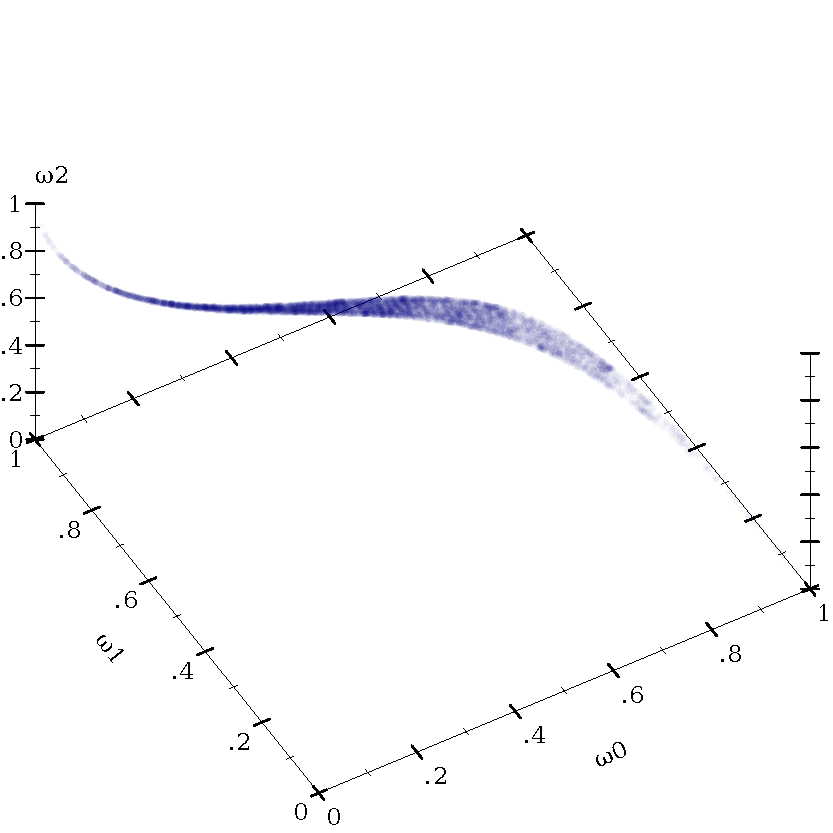
\includegraphics[width=\subfigurewidth]{results/normal-normals-wide1-points}%
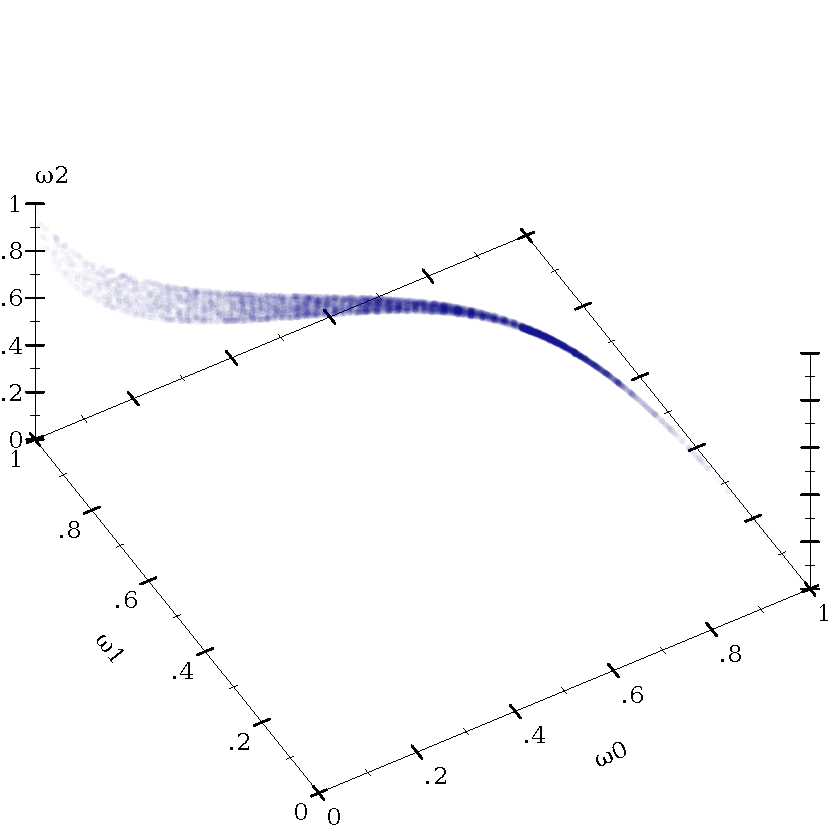
\includegraphics[width=\subfigurewidth]{results/normal-normals-wide2-points}%
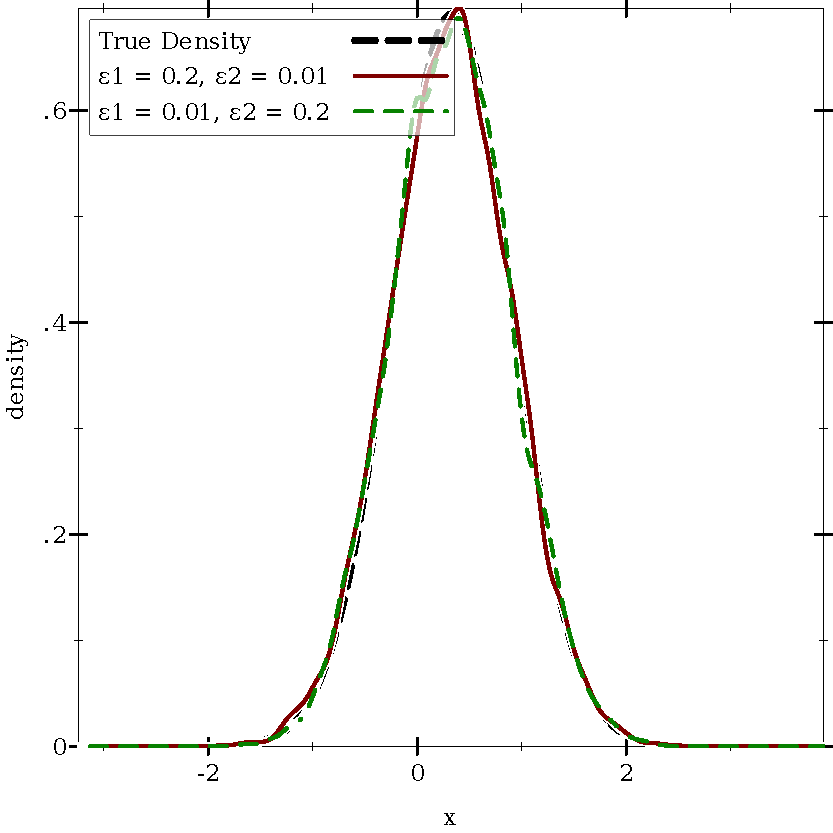
\includegraphics[width=\subfigurewidth]{figures/normal-normals-density}%
\caption[Inference with $\varepsilon_i$ of differing magnitudes]{From left to right, samples from the preimage of a condition using $\varepsilon_1 = 0.2,\varepsilon_2 = 0.01$, samples using $\varepsilon_1 = 0.01,\varepsilon_2 = 0.2$, and density estimates computed from the images of the sets of samples.}%
\label{fig:normal-normals}
\end{figure*}

Rudin's example suggests something that is possibly counterintuitive, but fortunate: that a wide observation $\mathit{Y_1} \in [y_1-0.2,y_1+0.2]$ may affect the distribution of $\mathit{X}$ as much as a narrow observation $\mathit{Y_2} \in [y_2-0.01,y_2+0.01]$.
Figure~\ref{fig:normal-normals} demonstrates precisely this using the \scheme{normal-normals} template with two observations $y_1 := 2$ and $y_2 := -1$, all standard deviations set to $1$, and two different settings for $\varepsilon_1,\varepsilon_2$.
The left plot shows 10000 samples from the preimage using $\varepsilon_1 = 0.2,\varepsilon_2 = 0.01$.
The middle plot shows 10000 samples using $\varepsilon_1 = 0.01,\varepsilon_2 = 0.2$.
Though the preimage sets are visibly different, $\mathit{X}$'s estimated density is nearly the same either way: close to the true distribution, a normal with $\mu = \frac{1}{3}$ and $\sigma = \sqrt{\frac{1}{3}}$.
In both cases, the $\mu$ estimate's Monte Carlo standard deviation is about $0.006$.

\subsection{Polynomial Fitting}

When encoding and computing conditional queries about normal-normal theories, it is easy to notice that the time it takes Dr. Bayes to sample is superlinear in the number of observations.
In fact, this is expected.
Because $\Omega$ subsets are represented by trees that correspond with the expression tree and projections are looked up and updated starting from the root, a \scheme{(random)} expression's image and preimage computation takes time proportional to its depth in the fully inlined program.
Because \scheme{(list e$_1$ e$_2$ ... e$_n$)} is equivalent to \scheme{(cons e$_1$ (cons e$_2$  (cons ... (cons e$_n$ null)))}, if each \scheme{e$_i$} has one \scheme{(random)} subexpression at a constant depth, its overall time complexity is $O(n^2)$.

We are fine with this for now.
At this early stage, theoretical simplicity is more important than speed.
Additionally, it gives us a fresh problem on which to demonstrate using Dr. Bayes for Bayesian regression, particularly to infer the distribution of a random function from number of observations to running time.

\begin{lrbox}{\codebox}
\begin{varwidth}{\textwidth}
\begin{center}\singlespacing
\begin{schemedisplay}
(define ns  (list     0     1     2     3     4     5     6     7 ...))
(define ts* (list 0.063 0.262 0.493 0.814 1.222 1.708 2.238 2.883 ...))
<blank-line>
(define/drbayes (quadratic-eval a0 a1 a2 n)
  (+ a0 (* n (+ a1 (* n a2)))))
<blank-line>
(define/drbayes (generate a0 a1 a2 ns)
  (if (null? ns) null (cons (normal (quadratic-eval a0 a1 a2 (first ns)) 1)
                            (generate a0 a1 a2 (rest ns)))))
<blank-line>
(define/drbayes (condition ts ts*)
  (if (null? ts) #t (and (let ([t   (first ts)]
                               [t*  (first ts*))])
                           (<= (- t* 0.001) t (+ t* 0.001)))
                         (condition (rest ts) (rest ts*)))))
<blank-line>  
(define/drbayes normal-normal-running-time
  (let* ([a0  (cauchy 0 0.1)]
         [a1  (cauchy 0 0.1)]
         [a2  (cauchy 0 0.1)]
         [ts  (generate a0 a1 a2 ns)])
    (list a0 a1 a2 (condition ts ts*))))
\end{schemedisplay}
\end{center}
\vspace{-0.75\baselineskip}
\hrule
\end{varwidth}
\end{lrbox}

\begin{figure*}[p!]\centering%
\subfloat[A Bayesian theory of the running time of Dr. Bayes as a quadratic function of the number of observations.]{%
\label{fig:quadratic-fit-bayesian:program}
\usebox{\codebox}
}

\subfloat[The observations, sampled quadratic polynomials given observations, and a $95\%$ confidence interval for the average quadratic polynomial.]{%
\label{fig:quadratic-fit-bayesian:plots}
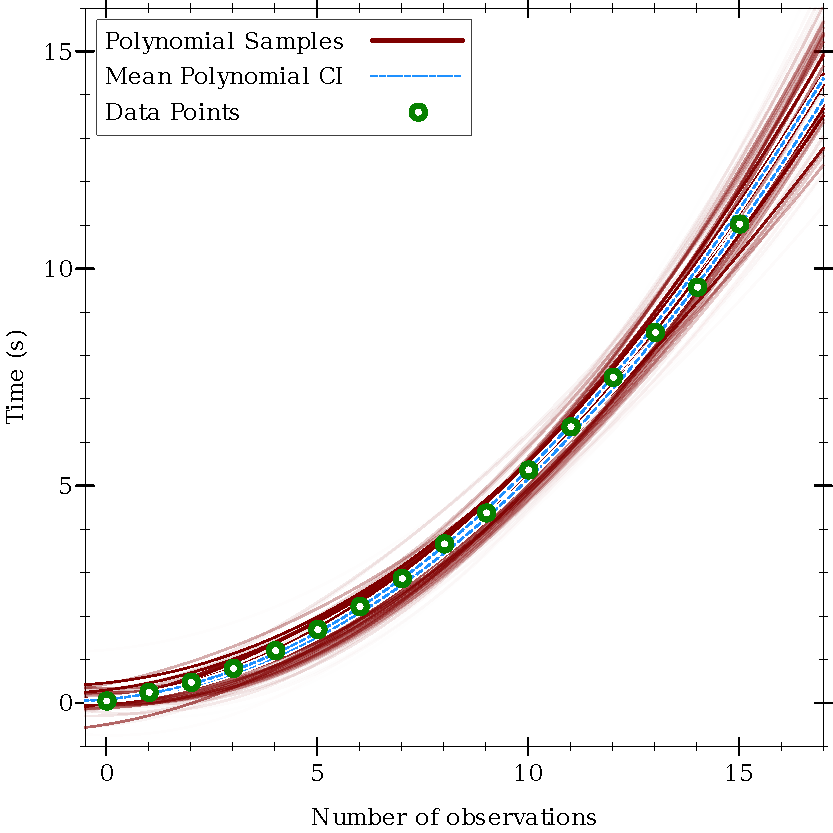
\includegraphics[width=3in]{figures/quadratic-fit-bayesian}%
\tab%
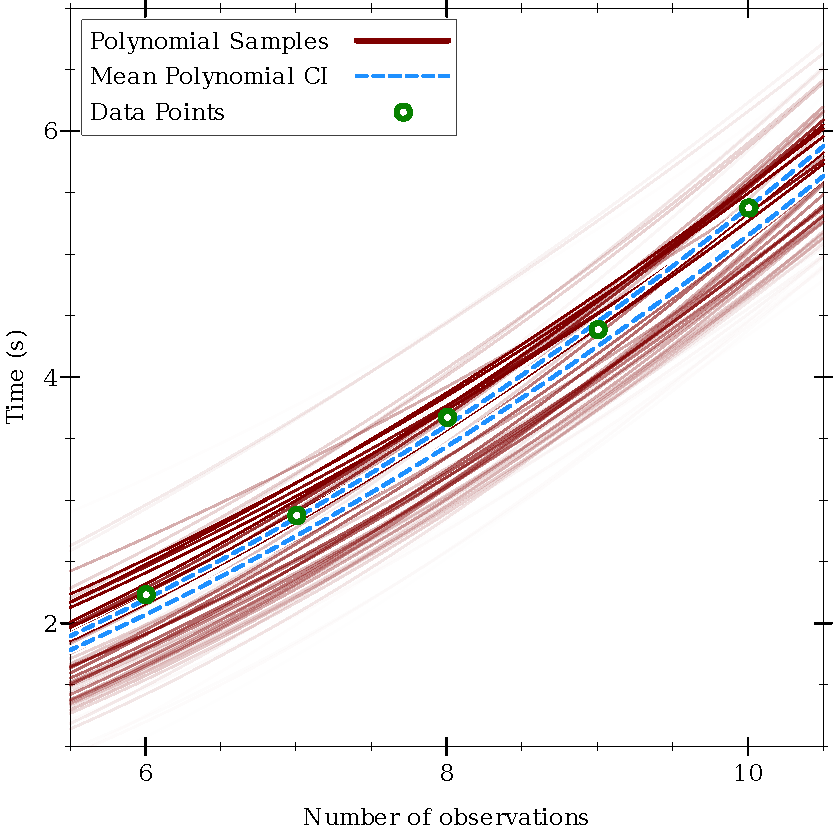
\includegraphics[width=3in]{figures/quadratic-fit-bayesian-zoom}%
}
\caption[Bayesian analysis of Dr. Bayes's running time, using Dr. Bayes]{Bayesian analysis of Dr. Bayes's running time, using Dr. Bayes.}%
\label{fig:quadratic-fit-bayesian}
\end{figure*}

Figure~\ref{fig:quadratic-fit-bayesian} demonstrates using Dr. Bayes to reason about the behavior of Dr. Bayes.
The theory is as follows: let $a_0,a_1,a_2$ be random coefficients that define a quadratic function $f~n := a_0 + a_1 \cdot n + a_2 \cdot n^2$, where $n$ is the number of observations.
We assume that the time to take $1000$ samples conditioned on $n$ observations is $f~n$ seconds plus some normally distributed noise.
We are interested in the distribution of $f$ (equivalently the distribution of $\pair{a_0,a_1,a_2}$) given some running time observations.

A priori, we do not know much about $a_0$, $a_1$ and $a_2$, so we assume they have Cauchy distributions, which are bell-shaped like normal distributions but allow much more variation.
We also allow the random noise added to $f~n$ to be fairly large (standard deviation $1$ second).

We collected running times for $0$ through $15$ observations with millisecond accuracy.
This data is encoded as \scheme{ns} (numbers of observations) and \scheme{ts*} (observed times) in Figure~\ref{fig:quadratic-fit-bayesian:program}.
The function \scheme{quadratic-eval} evaluates $f$.
The \scheme{generate} function returns a list of running time random variables generated from \scheme{ns}.
The \scheme{condition} function returns a boolean random variable which is \scheme{#t} only when every \scheme{t} in \scheme{ts} is near its corresponding observation \scheme{t*} in \scheme{ts*}.
Because our times have millisecond accuracy, \scheme{condition} requires each \scheme{t} to be within a millisecond of \scheme{t*}, or it returns \scheme{#f}.

The encoding of our theory outputs a list containing $a_0$, $a_1$, $a_2$ and the value of the condition.
Sampling within the preimage of $\Re \times \Re \times \Re \times \set{true} \times \set{\pair{}}$, and taking the image of these samples, results in samples from the distribution of $f$'s coefficients given the observations.

Figure~\ref{fig:quadratic-fit-bayesian:plots} shows two views of a plot of the observations, the polynomial function samples, and an inferred $95\%$ confidence interval computed by fitting a normal distribution to the computed mean of each coefficient and its Monte Carlo standard deviation.
By our prior knowledge and the close fit, we believe the quadratic model is a good one.

In fact, we will use it to make a prediction.
By evaluating each sampled quadratic polynomial on $n = 50$, we get samples from a distribution over running times with mean $113.5$ and standard deviation $15.6$.
The distribution's upper and lower $2.5\%$ quantiles are approximately $83$ and $144$; thus, if the model is correct, then given the observations, there is a $95\%$ probability that the running time for $50$ normal-normal observations is between approximately $83$ and $144$ seconds.
When we test this prediction (i.e. sample under the normal-normal theory with $50$ observations), Dr. Bayes takes $141.5$ seconds.

\subsection{Model Selection}

When Bayesian practitioners have two or more competing theories in mind to explain some phenomenon, they perform \keyword{model selection} to determine which is most probable.
Of course, we call it \mykeyword{theory selection}.

As a constructive theory, selecting between two theories is
\mathversion{normal}
\begin{equation}
\begin{aligned}
	&M \ \sim\ [m_1 \mapsto p_1, m_2 \mapsto p_2] \\
	&\begin{aligned}
	&\Theta \ \sim\ 
		\begin{cases}
			\mathrm{Prior_1} & \text{if } M = m_1 \\
			\mathrm{Prior_2} & \text{if } M = m_2
		\end{cases}
	\end{aligned}
	&\tab\tab
	\begin{aligned}
	&Y \ \sim\ 
		\begin{cases}
			\mathrm{Likelihood_1}(\Theta) & \text{if } M = m_1 \\
			\mathrm{Likelihood_2}(\Theta) & \text{if } M = m_2
		\end{cases}
	\end{aligned}
\end{aligned}
\end{equation}
where $p_1$ and $p_2$ are the probabilities of theories $m_1$ and $m_2$, and $\Theta$ is a random vector of parameters for one theory or the other.
A concrete, though contrived example is
\begin{equation}
\begin{aligned}
	&M \ \sim\ [\mathit{cc} \mapsto \tfrac{1}{2}, \mathit{nn} \mapsto \tfrac{1}{2}] \\
	&\begin{aligned}
	&X \ \sim\ 
		\begin{cases}
			\mathrm{Cauchy}(0,1) & \text{if } M = \mathit{cc} \\
			\mathrm{Normal}(0,1) & \text{if } M = \mathit{nn}
		\end{cases}
	\end{aligned}
	&\tab\tab
	\begin{aligned}
	&Y \ \sim\ 
		\begin{cases}
			\mathrm{Cauchy}(X,1) & \text{if } M = \mathit{cc} \\
			\mathrm{Normal}(X,1) & \text{if } M = \mathit{nn}
		\end{cases}
	\end{aligned}
\end{aligned}
\end{equation}
Here, the competing theories are Cauchy-Cauchy and normal-normal.

The major task in theory selection is computing the distribution of $M \given Y = y$, to determine the probabilities of each theory given observed data.
Theoretically, it is as simple as applying a version of Bayes' law for mixed masses and densities:\footnote{Technically, every version of Bayes' law that Bayesians use is Bayes' law for Radon-Nikod\'ym derivatives.} if $f_Y(y) > 0$, then
\begin{equation}
\begin{aligned}
	p_{M|Y}(m \given y)&\ =\ \frac{p_{M}(m) \cdot f_{Y|M}(y \given m)}{f_{Y}(y)}
\\
	&\ =\ \frac{p_{M}(m) \cdot f_{Y|M}(y \given m)}{\displaystyle\sum_{m \in \set{m_1,m_2}} p_{M}(m) \cdot f_{Y|M}(y \given m)}
\end{aligned}
\end{equation}
Unlike using Bayes' law for densities in Chapter~\ref{ch:background}, this is \emph{not} conveniently in terms of functions we have on-hand.
While we have $p_M = [m_1 \mapsto p_1, ..., m_n \mapsto p_n]$, we do not have the conditional density $f_{Y|M}$.
Much of the literature on Bayesian theory selection is devoted to efficiently computing $f_{Y|M}$ or approximations of it that can be used in certain circumstances.

Combining theories with density models results in a theory with a density model.
Sometimes the combined density model is amenable to traditional Monte Carlo methods.
(An example is our contrived Cauchy-Cauchy vs. normal-normal theory.)
Practitioners then need only sample according to the density conditioned on the data, and count the frequencies with which $M = m_1$, $M = m_2$ and so on.

\mathversion{sans}

In Dr. Bayes, that always works.
For example, suppose we want to determine whether Dr. Bayes's normal-normal running time is best modeled by a distribution over quadratic functions $f~n := a_0 + a_1 \cdot n + a_2 \cdot n^2$ or exponential functions $g~n := b_0 + b_1 \cdot 2^n$.
As with $a_0$, we assume $b_0$ has a Cauchy distribution.
But $b_1$ should not be negative and we do not expect it to be large, so instead of a Cauchy distribution, we assume it has an exponential distribution with scale $\tfrac{1}{2}$.
A priori, we assume the quadratic and exponential theories are equally likely.

\begin{lrbox}{\codebox}
\begin{varwidth}[b]{\textwidth}
\def\oldcodesize{\codesize}
\def\codesize{\small}
\begin{center}\singlespacing
\begin{schemedisplay}
(define/drbayes quad-or-exp-running-time
  (if (< (random) 1/2)
      ;; Quadratic running time
      (let* ([a0  (cauchy 0 0.1)]
             [a1  (cauchy 0 0.1)]
             [a2  (cauchy 0 0.1)]
             [ts  (generate-quad a0 a1 a2 ns)])
        (list #t (list a0 a1 a2)
              (condition ts ts*)))
      ;; Exponential running time
      (let* ([b0  (cauchy 0 0.1)]
             [b1  (exponential 0.5)]
             [ts  (generate-exp b0 b1 ns)])
        (list #f (list b0 b1)
              (condition ts ts*)))))
\end{schemedisplay}
\end{center}
\def\codesize{\oldcodesize}
\end{varwidth}
\end{lrbox}


\begin{figure*}[tb!]\centering
\subfloat[Encoding of Bayesian theory selection]{
\usebox{\codebox}
}
\tab
\subfloat[Data points and sampled running time functions]{
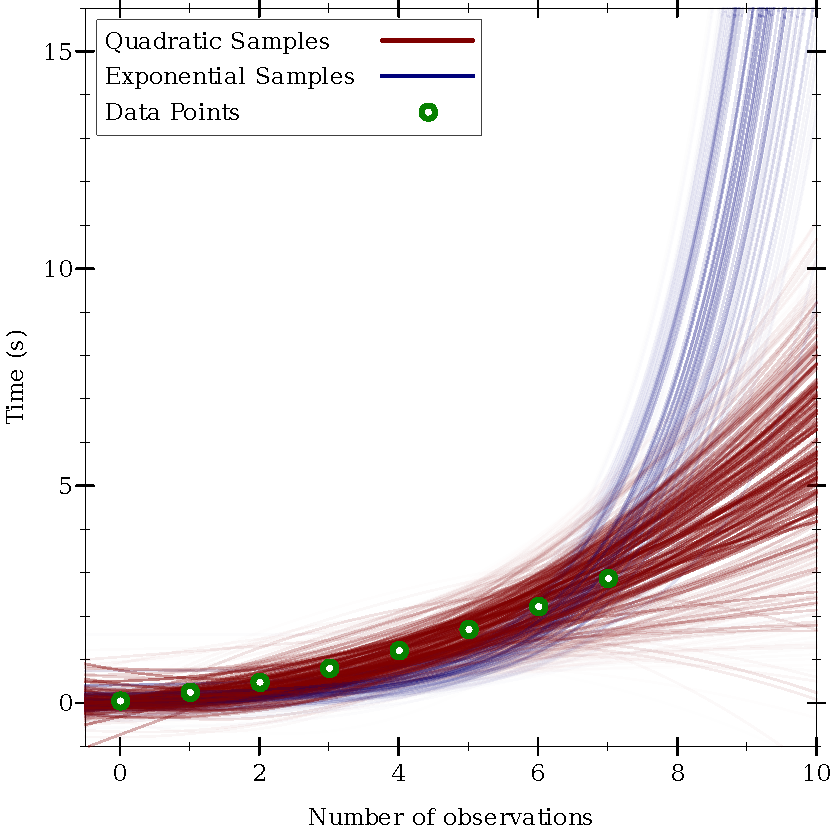
\includegraphics[width=3in]{figures/model-selection}
}
\caption[Bayesian theory selection in Dr. Bayes]{Bayesian theory selection in Dr. Bayes.}
\label{fig:model-selection}
\end{figure*}

Figure~\ref{fig:model-selection} shows some of the encoding of the combined theory.
(The rest is similar to \scheme{quadratic-eval} and \scheme{generate} in Figure~\ref{fig:quadratic-fit-bayesian:program}.)
It also shows the results of sampling in the conditioned model.
We use only $8$ observations, as adding more makes the exponential theory too unlikely; for example, a typical run with $16$ observations returns no exponential function samples.
With $8$ observations, we compute
\begin{center}\singlespacing
\begin{schemedisplay}
> (real-dist-hpd-interval
   (mc-prob-dist (λ (m) m) ms ws)
   0.95)
0.8543205426853948
0.8858619943029161
\end{schemedisplay}
\end{center}
where \scheme{ms} is the list of boolean theory choices, in which \scheme{#t} represents choosing quadratic.
Thus, we are $95\%$ confident that the probability of the quadratic theory, given the $8$ observations, is between $0.85$ and $0.89$.
Given $16$ observations, the probability of the quadratic theory is approximately $1$.


\section{Theories Without Density Models}

While Dr. Bayes has not yet constructed a density model for any of our theories, all of them so far have density models.
In this section, we demonstrate some useful theories that do not have density models.

\subsection{Bounded Measuring Devices}

The simplest theories without density models try to faithfully model measuring devices, which in reality cannot output unbounded values.

Suppose we wish to model a thermometer that would display the actual temperature with normally distributed noise, except that it cannot display numbers less than $0$ or greater than $100$.
Here is a theory in which we assume the true temperature is $\mathit{F}$:
\mathversion{normal}%
\begin{equation}
\begin{aligned}
	T' &\sim \mathrm{Normal}(F,1) \\
	T &= \max(0,\min(T',100))
\end{aligned}
\end{equation}
\mathversion{sans}%
A typically Bayesian task would be to infer the distribution of the outside temperature given a thermometer reading.
An encoding in Dr. Bayes is
\begin{center}\singlespacing
\begin{schemedisplay}
(define/drbayes temp-outside
  (let* ([temp   (normal 90 10)]
         [therm  (max 0 (min 100 (normal temp 1)))])
    (cons temp therm)))
\end{schemedisplay}
\end{center}
where \scheme{(normal 90 10)} represents our prior knowledge about the outside temperature.

\begin{figure*}[tb!]\centering%
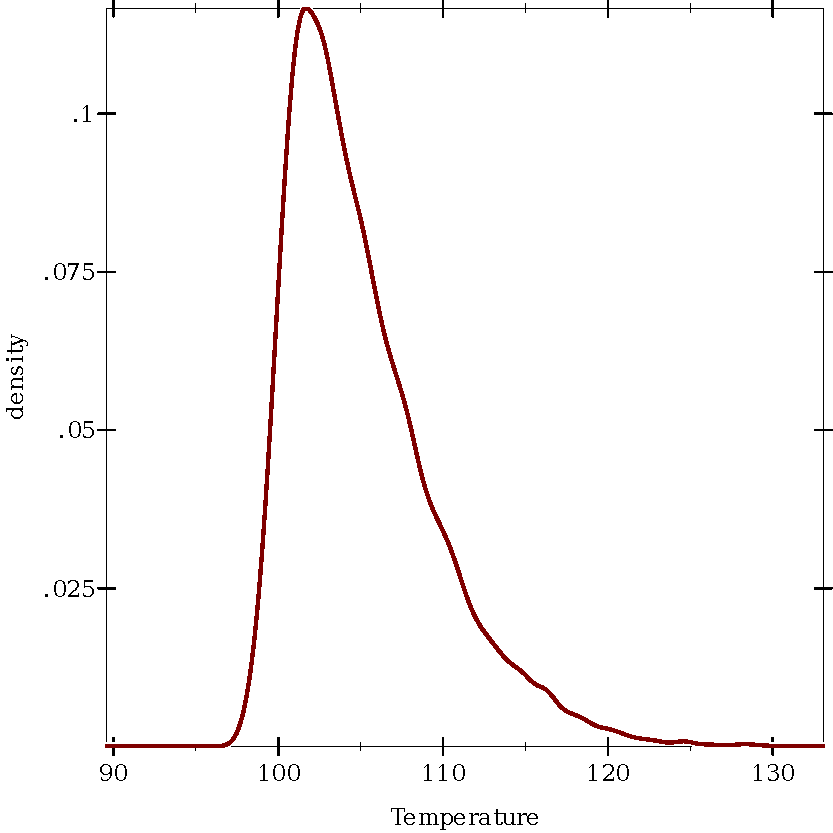
\includegraphics[width=3.5in]{results/thermometer-density}%
\caption[Bayesian inference with a bounded measuring device]{Distribution over temperature given that our thermometer displays its maximum value $100$.}%
\label{fig:thermometer-results}
\end{figure*}

Suppose we see the thermometer pegged at $100$.
What is the distribution of the outside temperature?

Figure~\ref{fig:thermometer-results} plots a density estimate of the image of samples taken in the preimage of $\Re \times [100,100]$.
The distribution is skewed left, as we might expect: its mode is approximately $102$, and the temperatures below $102$ that can cause the thermometer to display $100$ have lower probability than the temperatures above $102$ that can cause it.
The distribution is wide, corresponding with the fact that reading the maximum value does not tell us much about the probability of temperatures above the maximum value.

With $95\%$ probability, the outside temperature is between about $98.4$ and $114.5$:
\begin{center}\singlespacing
\begin{schemedisplay}
> (real-hpd-interval 0.95 temps ws)
98.47185450009886
114.45483575358433
\end{schemedisplay}
\end{center}
As the result of a random simulation, these are of course random variables.
But they are not expected values, so it is more difficult to quantify uncertainty in them.\footnote{Quantifying uncertainty about HPD intervals requires more complicated methods than we have discussed, such as bootstrapping.}
Still, the mean's Monte Carlo standard deviation is about $0.047$, which indicates that they should be close to the true HPD interval.

While it may seem useless to infer that we know very little, it is in these cases that Bayesian inference shines.
In low-knowledge situations, prior knowledge becomes more important.
Because Bayesian theories explicitly represent prior knowledge, inference can fill in the gaps.
See, for instance, Toronto et al~\cite{cit:toronto-2009cvpr}, wherein defaced portions of a photograph are marked as missing data (i.e. no knowledge).
A prior distribution that weakly favors continuous edges and contiguous color regions allows inference to fill in the missing data quite accurately.
This work in particular, which tries to faithfully model the process of taking a photograph, could have benefited from not requiring a density model, to account for the fact that each camera sensor, at each image location, is a bounded measuring device.
If it had, inference could have found plausible shapes in under- and overbright portions of photographs, and could have been used to undo sensor saturation and fix blooming artifacts.


\subsection{Non-Axial Conditions}

Faithfully modeling the process of taking a photograph also requires non-axial conditions.
The quantity measured by each sensor is a weighted sum of random quantities that represent light arriving from slightly different directions.
Observing such sums amounts to conditioning on hyperplanes.
In general, the result of asserting these and other non-axial, zero-probability conditions must be a measure-theoretic model, not a density model.

\begin{figure*}[tb!]\centering%
\subfloat[$42144$ samples from the distribution of {$\mathit{X},\mathit{Y} \given \sqrt{\mathit{X}^2+\mathit{Y}^2} \in [1-\varepsilon,1+\varepsilon]$}, overlaid on a contour plot of the unconditioned density model]{%
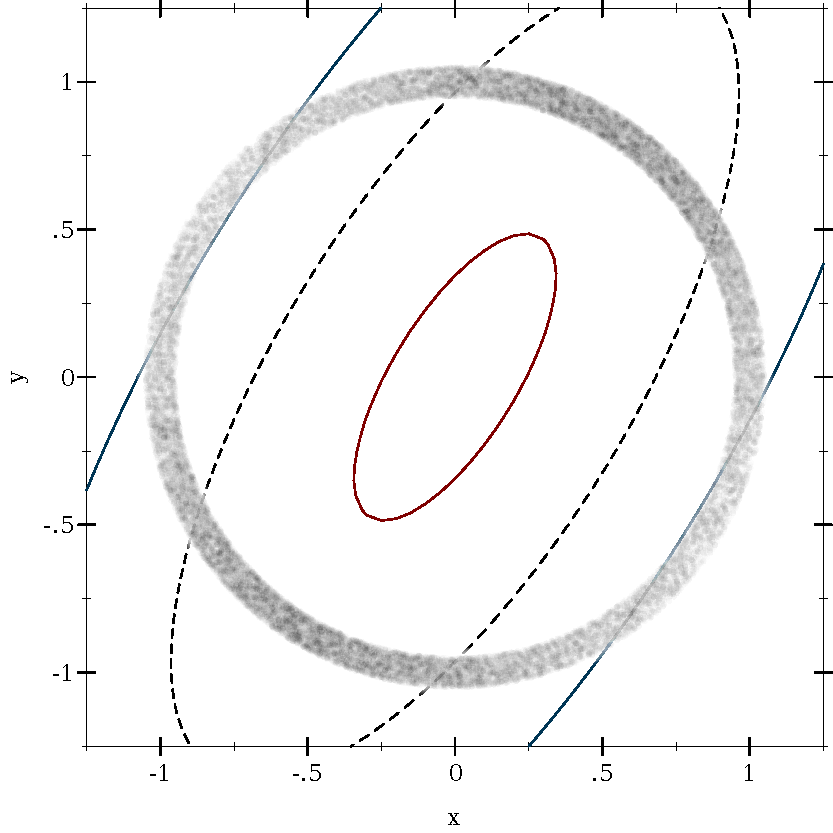
\includegraphics[width=3in]{results/circular-condition-image-points}%
}
\tab\tab\tab
\subfloat[Density estimate of the distribution of {$\mathit{X} \given \sqrt{\mathit{X}^2+\mathit{Y}^2} \in [1-\varepsilon,1+\varepsilon]$}]{%
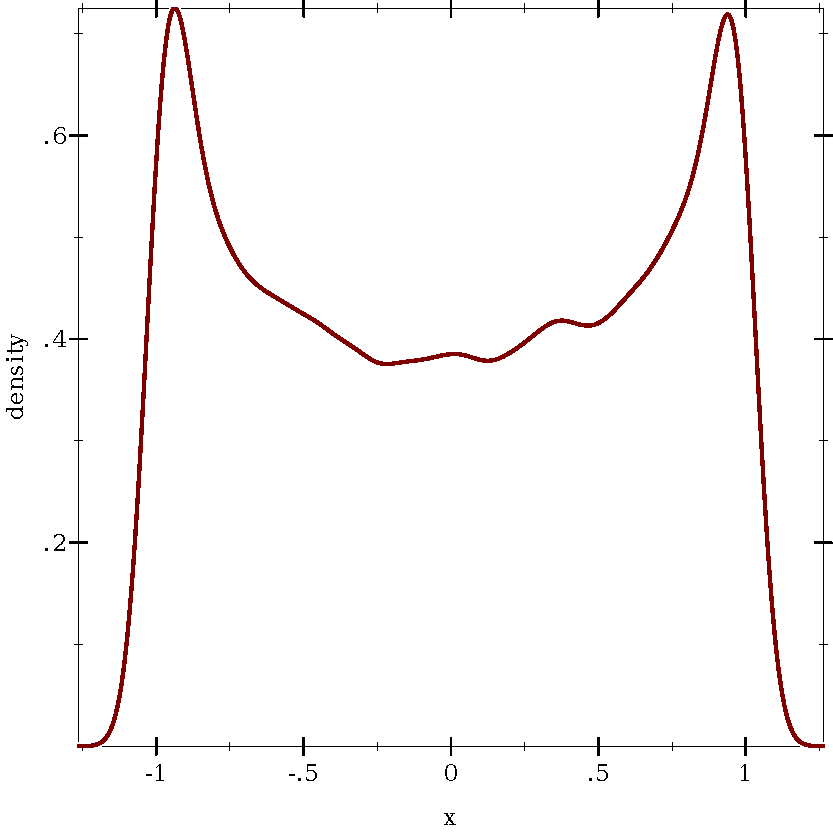
\includegraphics[width=3in]{results/circular-condition-density}%
}
\caption[Circular probabilistic conditions]{Sampling within circular probabilistic conditions.}%
\label{fig:circular-condition-results}
\end{figure*}

The next example conditions on something a little more difficult than sums.
Suppose we augment our normal-normal theory encoding with the distance from the origin:
\begin{center}\singlespacing
\begin{schemedisplay}
(define/drbayes normal-normal/distance
  (let* ([x  (normal 0 1)]
         [y  (normal x 1)])
    (list x y (sqrt (+ (sqr x) (sqr y))))))
\end{schemedisplay}
\end{center}
Figure~\ref{fig:circular-condition-results} shows the results of sampling within the preimage of $\Re \times \Re \times [1-\varepsilon,1+\varepsilon] \times \set{\pair{}}$, where $\varepsilon = 0.05$.
We are therefore conditioning on \scheme{x} and \scheme{y} being close to the unit circle.

We use $\varepsilon = 0.05$ to make the left plot's circular band of samples wide, so it is obvious that the point densities correspond with the density model for \scheme{normal-normal/distance}.
Dr. Bayes samples just as efficiently for any $\varepsilon > 0$.
Therefore, while in the limit as $\varepsilon$ approaches zero there is no density model, Dr. Bayes can still compute converging sequences of answers to queries.

We requested $50000$ samples and received $42144$.
The rejected samples are from sampling within overapproximations, which sometimes causes preimage refinement to return $\emptyset$.
We illustrate why further on.


\subsection{Stochastic Ray Tracing}

\begin{figure*}[!tb]\centering
\smallmathfont
\subfloat[Random paths from a single light source, conditioned on passing through an aperture]{
\begin{minipage}[b]{0.49\textwidth}
\centering
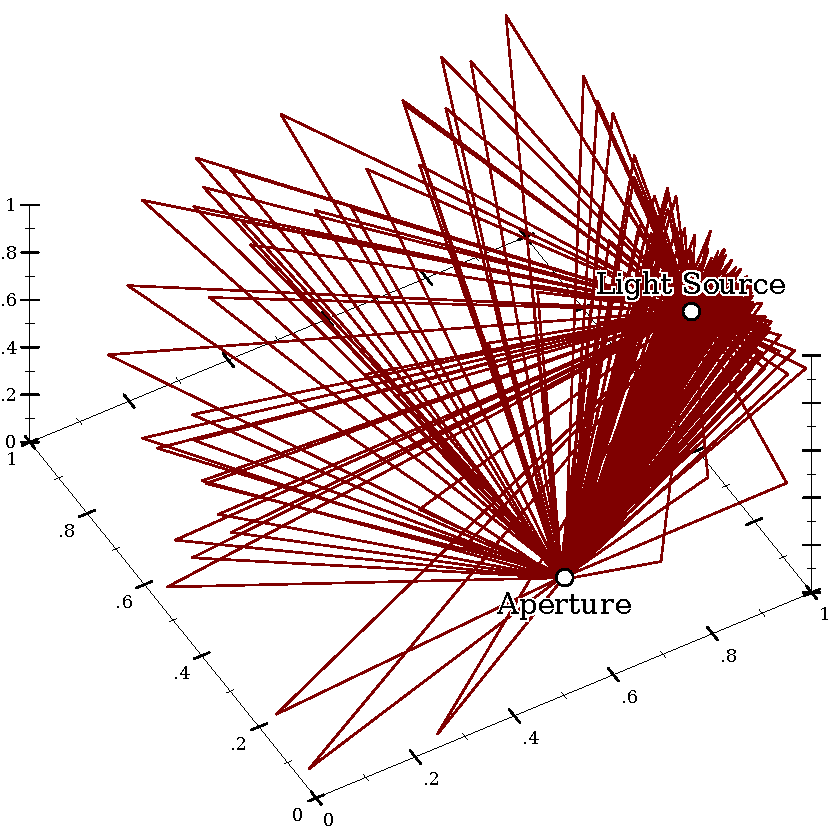
\includegraphics[width=\textwidth]{figures/ray-tracing}
\end{minipage}
\label{fig:ray-tracing-paths}
}
\tab\tab
\subfloat[Random paths that pass through the aperture, projected onto a plane and accumulated]{
\begin{minipage}[b]{0.43\textwidth}
\centering
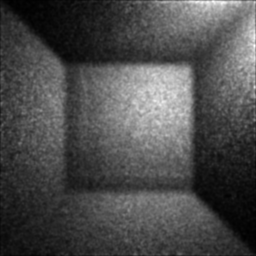
\includegraphics[width=\textwidth]{figures/ray-tracing-projection}
\end{minipage}
\label{fig:ray-tracing-projection}
}
\caption[Stochastic ray tracing in Dr. Bayes]{Stochastic ray tracing in Dr. Bayes.}
\label{fig:ray-tracing}
\end{figure*}

By implementing a small vector math library and some collision detection functions, we can encode a simple theory of light transport in Dr. Bayes for which conditional queries carry out stochastic ray tracing~\cite{cit:veach-1997siggraph-mlt}.
For example, the following functions compute the dot product between two vectors (represented by lists), and return a random vector with a uniform direction (for emitting light).
\begin{center}\singlespacing
\begin{schemedisplay}
(define/drbayes (vec-dot v1 v2)
  (+ (* (list-ref v1 0) (list-ref v2 0))
     (* (list-ref v1 1) (list-ref v2 1))
     (* (list-ref v1 2) (list-ref v2 2))))
<blank-line>
(define/drbayes (uniform-vec)
  (list (normal) (normal) (normal)))
\end{schemedisplay}
\end{center}
We have also implemented \scheme{vec-add}, \scheme{vec-neg} (negation) and \scheme{vec-scale} (elementwise multiplication by a constant).
We additionally define a structure to represent collisions:
\begin{center}\singlespacing
\begin{schemedisplay}
(struct/drbayes collision (time point normal))
\end{schemedisplay}
\end{center}
and a function to compute ray-plane intersections:
\begin{center}\singlespacing
\begin{schemedisplay}
(define/drbayes (ray-plane-intersect p0 v n d)
  (let ([denom  (- (vec-dot v n))])
    (if (positive? denom)
        (let ([t  (/ (+ d (vec-dot p0 n)) denom)])
          (if (positive? t) (collision t (vec-add p0 (vec-scale v t)) n) #f))
        #f)))
\end{schemedisplay}
\end{center}

Figure~\ref{fig:ray-tracing-paths} illustrates the main idea behind stochastic ray tracing.
Using the vector functions, we simulate casting photons uniformly from a light source and reflect them uniformly when they collide with the walls of a square room, which generates paths.
We condition on the paths passing through a small aperture, collect samples, and project them onto a collector plane on the other side of the aperture.
Figure~\ref{fig:ray-tracing-projection} shows the result of accumulating the collisions on the collector.
The smaller the aperture, the smaller the probability a path passes through it, and the more focused the resulting image.

All efficient implementations of stochastic ray tracing to date use sophisticated, specialized sampling methods that bear little resemblance to the physical processes they simulate.
The proof-of-concept ray tracer in Dr. Bayes is little more than a simple physics simulation and a conditional query.


\subsection{Probabilistic Program Verification}

If we recast probabilistic program verification~[XXX: cite] as ``find the distribution over program inputs given an error condition,'' it is equivalent to Bayesian inference.
To use Dr. Bayes to compute this conditional distribution for a given program, we
\begin{enumerate}
	\item Encode the program in Dr. Bayes in a way that propagates errors.
	\item Compute an overapproximation of the preimage of an error condition.
	\item Sample points in the overapproximation that are also in the preimage.
\end{enumerate}
Sometimes step 2 returns $\emptyset$, in which case there are no preconditions that produce errors (if the program is encoded correctly).
The longer the probabilistic search in step 3 runs without finding a point in the preimage set, the likelier it is that the preimage has zero probability or is empty.
The probabilistic search is guided by preimage computation to find errors, and can be guided further by manually adjusting the distribution over inputs.

Because dependent uniform sampling (i.e. $sample!source^*$ as defined in~\eqref{eqn:sample-source*}) is so sensitive to floating-point error, we are most interested in verifying error bounds for the outputs of floating-point implementations of real functions.

While Dr. Bayes's numbers are implemented by floating-point intervals, semantically, they are real numbers.
We therefore cannot represent floating-point numbers directly in Dr. Bayes---but we do not want to.
We need to represent \emph{abstract} floating-point numbers, consisting of an exact, real number and a bound on the relative error with which it is approximated.
We regard numbers with catastrophic relative error (i.e. not in $[0,1)$) as representing any floating-point number, and so define the following two structures.
\begin{center}\singlespacing
\begin{schemedisplay}
(struct/drbayes float-any ())
(struct/drbayes float (value error))
\end{schemedisplay}
\end{center}
An abstract value \scheme{(float v e)} represents every floating-point number between \scheme{(* v (- 1 e))} and \scheme{(* v (+ 1 e))} inclusive.

Abstract floating-point functions compute exact results and use input error to bound output error:
\begin{center}\singlespacing
\begin{schemedisplay}
(define/drbayes (flsqrt x)
  (if (float-any? x)
      x
      (let ([v  (float-value x)]
            [e  (float-error x)])
        (cond [(negative? v)  (float-any)]  ; NaN
              [(zero? v)      (float 0 0)]  ; exact case
              [else
               ; v is positive
               (make-float (sqrt v)                   ; exact square root
                           (+ (* 1/2 epsilon.0)       ; rounding error
                              (- 1 (sqrt (- 1 e)))))  ; exact relative error
              ]))))
\end{schemedisplay}
\end{center}
Here, \scheme{(make-float v e)} returns \scheme{(float-any)} when \scheme{(> e 1)}.
We have also implemented arithmetic and comparison operators, as well as exponentials and logarithms.

Suppose we define an abstract floating-point implementation of the geometric distribution family's inverse CDF:
\begin{center}\singlespacing
\begin{schemedisplay}
(define/drbayes (flgeometric-inv-cdf u p)
  (fl/ (fllog u) (fllog (fl- (float 1 0) p))))
\end{schemedisplay}
\end{center}
We want the distribution of \scheme{x} and \scheme{y} in $(0,1)$ given that the output error
\begin{center}
\begin{schemedisplay}
(float-error (flgeometric-inv-cdf (float x 0) (float y 0)))
\end{schemedisplay}
\end{center}
is in $(3 \cdot \varepsilon,+\infty)$, where $\varepsilon \approx 2.22\cdot 10^{-16}$ is the smallest 64-bit floating-point number that can be added to $1.0$ to yield a different floating-point number.
That is, we want the distribution of exact inputs for which the approximate output is more than about three floating-point numbers away from the exact output.\footnote{Floating-point functions are almost always analyzed assuming exact inputs. Few useful ones \emph{reduce} error.}

Dr. Bayes overestimates the preimage of $(3 \cdot \varepsilon,+\infty)$ as approximately $(0,1) \times (\varepsilon,0.284)$ and returns samples within it.
Knowing a few common floating-point tricks, we define
\begin{center}\singlespacing
\begin{schemedisplay}
(define/drbayes (flgeometric-inv-cdf u p)
  (fl/ (fllog u) (fllog1p (flneg p))))
\end{schemedisplay}
\end{center}
where \scheme{fllog1p} (abstractly) computes $log1p~x := log~(1+x)$ with high accuracy.
The preimage of $(3 \cdot \varepsilon,+\infty)$ is now $\emptyset$.
In fact, the preimage of $(1.51 \cdot \varepsilon,+\infty)$ is $\emptyset$, meaning that this implementation of \scheme{flgeometric-inv-cdf} returns approximations that are no more than about $1.51$ floating-point numbers away from the exact answers.

It would take more detailed abstractions of floating-point numbers to reason about subnormal numbers, NaNs, signed zeros, and infinities.


\section{Current Shortcomings}

To make progress, we must undertake the painful process of characterizing Dr. Bayes's shortcomings.
We do not believe any of them are insurmountable, so we regard them as a guide for future work.

\subsection{Engineering Required}

The simplest shortcomings require only engineering, and perhaps some numerical analysis.

With Dr. Bayes's current primitives, we can find no good way to encode the gamma distribution family, beta distribution family and Dirichlet distribution family, all of which are important in Bayesian practice.
Dr. Bayes needs a two-argument gamma primitive, from which these families can be defined.

The Bernoulli, multinomial, Poisson and geometric distribution families, and arbitrary discrete distributions can be encoded using \scheme{if} (or \scheme{strict-if}), \scheme{random}, \scheme{<}, and recursive functions.
The correctness and termination theorems for Dr. Bayes's semantics prove that programs using such encodings work as expected.
But defined this way, they are slow.

Bayesians tend to think in terms of propositions, not sets.
Encoding conditions as boolean expressions and sampling within the preimage of a rectangle with a $\set{true}$ axis is a good start, but Dr. Bayes should hide these details from users.

\subsection{Research May Be Required}

For some of Dr. Bayes's shortcomings, we do not know yet whether engineering work is sufficient.

When we encode theories as functions, we write them to return every random variable of interest in a list so we can estimate their expected values and study their behavior.
Theories assembled from many such functions are quite verbose because function applications must destructure lists of returned values.
It seems we need not just functions, but an additional form of abstraction that is more transparent by default.

Lambdas would make the encoding of the theory of quadratic running time in Figure~\ref{fig:quadratic-fit-bayesian} shorter.
The \scheme{generate} function would be an easy application of \scheme{map}, and \scheme{condition} an easy application of \scheme{andmap}.
Adding lambda expressions could be as simple as using well-known techniques for compiling higher-order languages to first-order target languages.

Errors are often hard to find.
Consider this bad program:
\begin{center}\singlespacing
\begin{schemedisplay}
(define/drbayes add-number-to-list
  (+ 1 (list (random))))
\end{schemedisplay}
\end{center}
If we try to sample, we get this unhelpful error message:
\begin{center}\singlespacing
\texttt{drbayes-sample: cannot sample from the empty set}
\end{center}
The culprit here is not distinguishing between errors and nontermination: for simplicity, they are both $\bot$ in the semantics.
In the exact semantics, computing preimages removes inputs that produce $\bot$, so errors do not occur.
To begin addressing this, Dr. Bayes needs a separate type of error values, as well as a representation for rectangular sets of error values.
We do not know whether exception handling is required or desirable, whether it makes sense to ignore errors that happen with zero probability, nor how difficult it is to distinguish between errors that arise only from overapproximation and those that are truly errors.

We have done inference on probabilistic context-free grammars specified very naturally as mutually recursive functions.
We did not demonstrate them because Dr. Bayes lacks symbols, so the languages consist of lists of \scheme{#t} and \scheme{#f}, making them hard to understand.
Dr. Bayes also does not have string and integer data types.
Lacking abstract sets of strings, we have encoded no theories containing string manipulation.
The obvious representation, rectangular products of sets of characters, may not be precise enough.

\subsection{Research Required}

Addressing the rest of Dr. Bayes's shortcomings will require quite a lot of research.

While Dr. Bayes is \emph{efficient}, in the sense that the time complexity of sampling is a polynomial of low degree, it is not fast.
In particular, the ray tracer takes around 10000 times the time a hand-coded MCMC sampler would take to produce the same number of samples.
Much of the slowdown comes from computing images and preimages for deep \scheme{(random)} expressions, which is quadratic in the depth of the expression.

The ray-traced image in Figure~\ref{fig:ray-tracing-projection} is accumulated from $20$ million samples.
The image is only $256 \times 256$, or $65536$ pixels, so it could be much less grainy.
The culprit is importance sampling, which often suffers from high Monte Carlo variance in high-dimensional spaces.

We could not set \scheme{drbayes-max-splits} to \scheme{5} before running the query that carried out stochastic ray tracing.
The search tree became too large to fit in memory.
The explosion in search tree size is similar to the state space explosion problem in model checking, and may be just as hard to solve.

Dr. Bayes repeats computations unnecessarily.
Consider this encoding of a theory of independent normal random variables:
\begin{center}\singlespacing
\begin{schemedisplay}
(define/drbayes independent-normals
  (let ([x  (normal 0 1)]
        [y  (normal 0 1)])
    (pair x y)))
\end{schemedisplay}
\end{center}
When $\Omega$ is split along the axis projected by \scheme{x}, Dr. Bayes carries out image and preimage computation for \scheme{y} as well, even though the results are the same as with the previous $\Omega$.
In fact, there is a good chance that in most programs, most $\Omega$ splits along one axis do not affect most image and preimage computations.

\renewcommand{\subfigurewidth}{2in}
\begin{figure*}[tb!]\centering
\subfloat[False independence causes loose rectangular cover fit]{%
\label{fig:dependency-problem:loose-fit}%
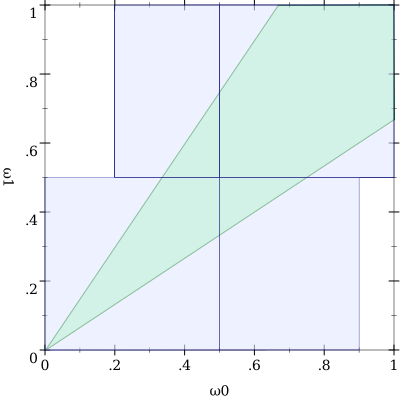
\includegraphics[width=\subfigurewidth]{figures/dep-problem}%
}%
\tab%
\subfloat[Nearly half of $\omega_0$ values on part cover sample result in rejection]{%
\label{fig:dependency-problem:rejection}%
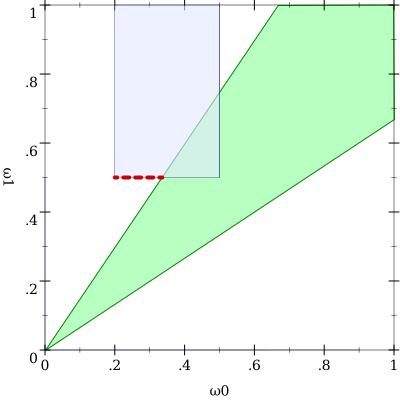
\includegraphics[width=\subfigurewidth]{figures/dep-problem-1}%
}%
\tab%
\subfloat[No false independence: tight fit, no rejections possible]{%
\label{fig:dependency-problem:tight-fit}%
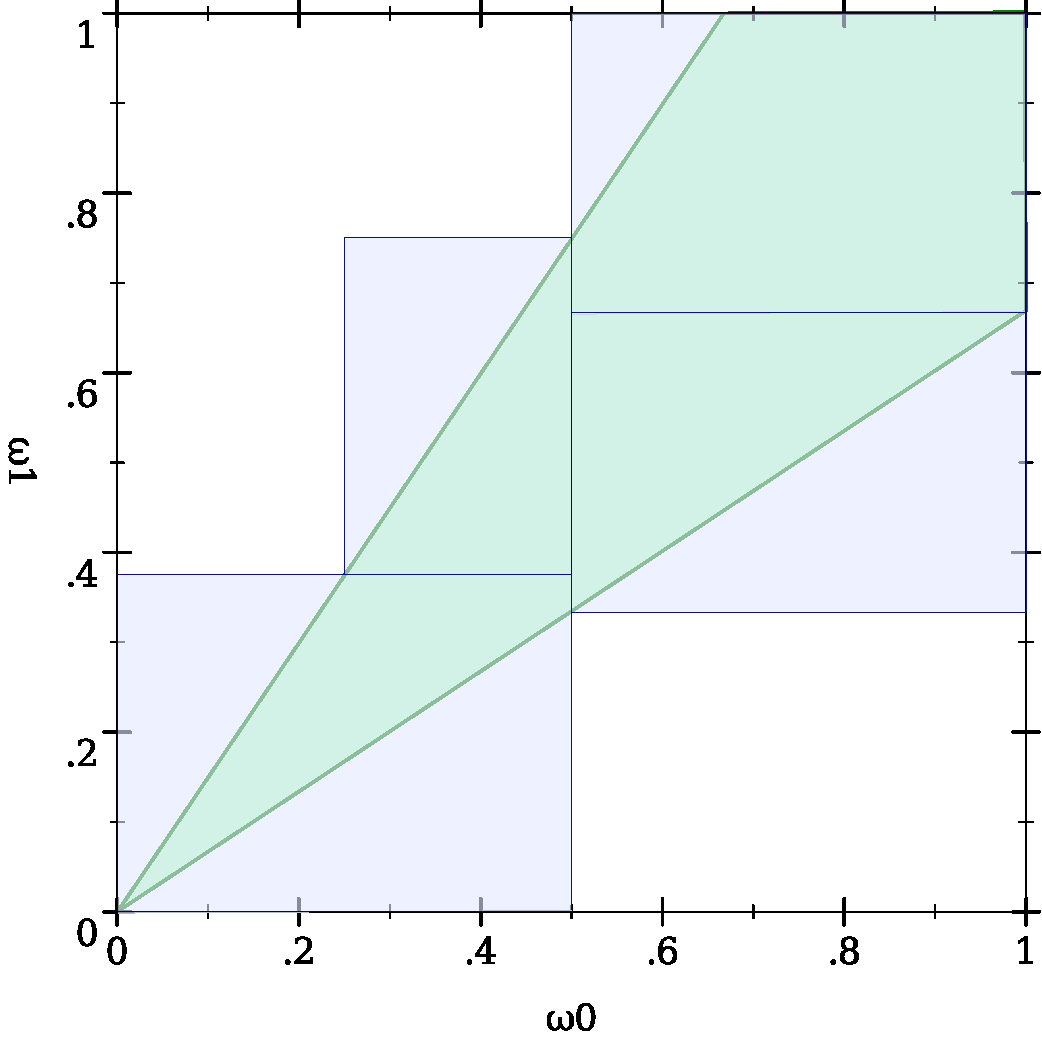
\includegraphics[width=\subfigurewidth]{figures/no-dep-problem}%
}%
\caption[The dependency problem]{The dependency problem: falsely assuming independence of variables that occur more than once in an expression causes the rectangular preimage cover to fit loosely.
If $\set{\omega_0}$ is drawn from the left of the part cover in (b), refinement returns $\emptyset$.}
\label{fig:dependency-problem}
\end{figure*}

For the normal-normal theory encoding with the circular condition, we requested 50000 samples and received 42144.
A much simpler program exhibits similar behavior:
\begin{center}\singlespacing
\begin{schemedisplay}
(define/drbayes dependency-problem
  (let ([x  (random)]
        [y  (random)])
    (/ x (+ x y))))
\end{schemedisplay}
\end{center}
Figure~\ref{fig:dependency-problem:loose-fit} shows the preimage of $[0.4,0.6]$ and the rectangular cover Dr. Bayes samples part covers from.
When it samples the part cover shown in Figure~\ref{fig:dependency-problem:rejection}, it fails about half the time because the part cover does not fit the preimage set as tightly as possible.

The loose fit happens because $x$ occurs twice in $x{/}(x+y)$, and image and preimage computation do not account for the fact that each $x$ occurrence refers to the same value.

To demonstrate how, we reason compositionally about its range.
Let $z := x + y$; then $z \in [0,2]$ because $x,y \in [0,1]$.
Because $\pair{x,z} \in [0,1] \times [0,2]$, $x{/}z \in [0,+\infty)$; therefore $x{/}(x+y) \in [0,+\infty)$.
Each of these statements is true---they even constitute a proof---so our reasoning is \emph{sound}.
But our reasoning is not \emph{precise}: it is not hard to show that $x{/}(x+y) \in [0,1]$.
In particular, $[0,1] \times [0,2]$ is a gross overestimate of the range of $\pair{x,z}$.

Just as in the preceeding proof that $x{/}(x+y) \in [0,+\infty)$, image and preimage computations are carried out compositionally and rectangles represent sets of possible values.
If \scheme{h} is the interpretation of \scheme{dependency-problem} as a preimage* arrow computation, we have
\begin{center}\singlespacing
\begin{schemedisplay}
> (pre-mapping-range ((h j0) program-domain))
(Real-Set 0.0 +inf.0 #t #f)
\end{schemedisplay}
\end{center}
In interval arithmetic, this is called the \keyword{dependency problem}.
The fact that preimages are restricted to domain \emph{parts} mitigates the problem somewhat.
We can mitigate it further by partitioning more finely, which works well enough but takes extra time and space.

We can occasionally solve the dependency problem by refactoring expressions.
For example, if $x \neq 0$, then $x{/}(x+y) = 1{/}(1+y{/}x)$.
In our program, $x \neq 0$ is a zero-probability event.
Therefore, as long as $x \neq 0$ is not an asserted condition, we can rewrite the program as
\begin{center}\singlespacing
\begin{schemedisplay}
(define/drbayes no-dependency-problem
  (let ([x  (random)]
        [y  (random)])
    (/ 1 (+ 1 (/ y x)))))
\end{schemedisplay}
\end{center}
without changing the meaning of any queries.
Figure~\ref{fig:dependency-problem:tight-fit} shows the resulting rectangular cover Dr. Bayes samples from, which tightly fits the preimage.

The dependency problem is not particular to interval arithmetic, but can be found in many kinds of abstract interpretation and static analysis.
As with using Monte Carlo methods instead of enumeration methods to compute preimage measures, we hope that providing only \emph{probabilistic} guarantees will make solving the problem more tractable.


\section{Conclusions}

Dr. Bayes is a proof-of-concept implementation, designed for exploring the expressive power and utility of the let-calculus whose semantics is defined in Chapter~\ref{ch:preimage1}.
We have shown that it is expressive enough to encode Bayesian theories with and without density models, including theories that (likely because they lack density models) are rarely regarded as Bayesian.
Even at this very early stage, as a mostly direct implementation of the semantics with barely any work put into making it fast, Dr. Bayes is useful, at least for problems with up to $25$ or so random variables.

We have demonstrated that allowing only positive-probability conditions matters little: they are philosophically easier to support, interval observations may be quite wide and still be as effectful as point observations, and interval observations' widths may be specified independently without affecting accuracy.

We have characterized Dr. Bayes's shortcomings and will use them to drive future work.


\mathversion{normal}

\begin{comment}
A summary of our position on why not supporting zero-probability conditions makes little difference is thus
\begin{itemize}
	\item Asserting zero-probability conditions overstates actual knowledge.
	\item Positive-probability observations can be fairly wide.
	\item Positive-probability observations can be entirely independent.
\end{itemize}
\end{comment}
